\documentclass{article}

\usepackage{amsthm}
\usepackage{amsfonts}
\usepackage{amsmath}
\usepackage{amssymb}
\usepackage[utf8]{inputenc}
\usepackage{graphicx}
\usepackage{fullpage}
\usepackage[usenames]{color}
\usepackage{hyperref}
  \hypersetup{
    colorlinks = true,
    urlcolor = blue,       % color of external links using \href
    linkcolor= blue,       % color of internal links 
    citecolor= blue,       % color of links to bibliography
    filecolor= blue,        % color of file links
    }
    
\usepackage{listings}

\definecolor{dkgreen}{rgb}{0,0.6,0}
\definecolor{gray}{rgb}{0.5,0.5,0.5}
\definecolor{mauve}{rgb}{0.58,0,0.82}

\lstset{frame=tb,
  language=haskell,
  aboveskip=3mm,
  belowskip=3mm,
  showstringspaces=false,
  columns=flexible,
  basicstyle={\small\ttfamily},
  numbers=none,
  numberstyle=\tiny\color{gray},
  keywordstyle=\color{blue},
  commentstyle=\color{dkgreen},
  stringstyle=\color{mauve},
  breaklines=true,
  breakatwhitespace=true,
  tabsize=3
}


\title{CPSC-354 Report}
\author{Joan Karstrom  \\ Chapman University}

\date{\today}

\begin{document}

\maketitle

\begin{abstract}
In CPSC 354, our class objective is to “have a look under the hood of programming languages.” Unlike other computer science courses, we are not focusing on learning a specific language, building huge repositories, and handling data. We are essentially comprehending *what* is a programming language and what do developers think of when they first are thinking of when designing a language. 

\medskip\noindent
Most of the time, we believe that the just syntax looks different, but there are so many more things to consider when choosing a language to program in. What hustles and benefits does the language have to offer you. In my report, I dive into Haskell, a purely functional programming language that is great for breaking down the blocks and simply showing the foundations of a language. Instead of creating programs with methods telling the computer what to do, Haskell allows you to say to the computer what *is*. Some theories of programming languages are also gone over in this report as we expand more of the grammar of languages. 
\end{abstract}

\tableofcontents

\section{Introduction}\label{intro}

This report is broken up into sections to better understand the material and better map how these topics are related. Overleaf was used on this report to format everything together, all cite hyperlinks should be live and working. 

\subsection{Haskell}

Haskell is a unique language and is very influential in understanding programming languages and the grammar of these languages that makes them so different. 

\medskip\noindent
As a student learning Haskell for the first time, a lot can be said about how one learns Haskell and how one can be successful in it.

\medskip\noindent
In the first section of this report names "Haskell", the basis of Haskell are covered, including a tutorial on what is needed to run Haskell and how to code in the language. 

\medskip\noindent
It also goes over a description of Haskell and what makes it different than other programming languages. And taking a look at a deeper understanding of why Haskell is formatted the way it is. 

\subsection{Programming Languages Theory}

In this section of the report, more is discussed about the building blocks of a programming language. Haskell is a great language to learn more about this concept by creating programs with custom grammar.

\medskip\noindent
Creating a programming language's grammar can limit and also expand a language.

\medskip\noindent
Parsing is an idea that is introduced when speaking about the grammar of a language which is explained further. In this class we created our own language based on Lambda Calculus.

\subsection{Project}

The last section of this report is the project. For my project, I looked at the Calculator I created as Assignment 1. I attempted to make an interface for the said application and also correcting past errors from the assignment.  

\medskip\noindent
I go more in depth in how I fixed the errors that I had with Assignment 1 and what is needed to further expand on the project. 

\medskip\noindent
I talk about the difficulties that I ran into for this assignment but also what I learned from the online interface creator for Haskell applications called IHP. This created a real time web page for the application.

\section{Haskell}\label{haskell}

Haskell is the base language that we were taught in this course. For a purely functional programming languages there are a lot of benefits.

\medskip\noindent
Haskell is completely free and can run on windows, macOS, and Linux. 

\medskip\noindent
 It has is very readable this is because of being Statically typed.I would compare it to python in some sense which I will expand on later in my report.
 
\medskip\noindent
It is also called a "purely functional" programming language which means it the functions in Haskell are all functional in the mathematical sense.\cite{HHP}. 

\medskip\noindent
Haskell's code is concise, and its syntax makes it easy to understand what you are coding, which means fewer mistakes.

\subsection{History of Haskell}
Haskell is a functional programming language that is used to learn and understand programming languages as it is used widely for research. 

\medskip\noindent
Before Haskell there was LISP which stood for List Processing which was one of the first high-level programming languages ever created.

\medskip\noindent
The development of this functional language started in 1987 by a 25 person committee formed by John Hughes, Philip Walder, Kevin Hammond, John Launchbury, and Simon Peyton Jones of people who attended the FPCA ‘87 conference. The “Haskell Report” was published in 1991 and since then has grown into a widely respected language \cite{HP}. 

\medskip\noindent
Glasgow Haskell Compiler is the most common Haskell compiler, it is named after the logician Haskell Curry.

\medskip\noindent
Haskell was created with the intent of research and teaching functional programming. It was a commonly used 'open sourced' language so that the community could be more together when conducting research. \cite{BHH} 

\medskip\noindent
There are only two official versions of Haskell, its most current version is Haskell 2011 but as of 2016 a group is working on building Haskell 2020.

\subsection{First Understanding}
Haskell was tough for me to understand at first. When first learning coding you are taught to use python, Java or CPP which are all syntactically similar. Haskell is a bit different from that and uses many recursions and theories that use discrete mathematics.

\medskip\noindent
When first learning Haskell I had to look up many tutorials to help me understand. Some tutorials that really helped me at first to start coding in Haskell was the website/blog "Learn You a Haskell" \cite{LH}. 

\medskip\noindent
When looking up outside resources to try and understand, I found that there were a lot of blogs teaching Haskell as it is not a very popular programming language. Reading people's own experience with the language helped ease my frustration with not understanding it at first, which seemed to be a common theme when first learning Haskell because of how different the language is. 

\medskip\noindent
I believe that this is more helpful than a book in the ways that it is explained in a way that I could better understand. It is less formal than a textbook, and sometimes these blogs would talk about how they first saw things and how they learned differently. 

\subsection{First Downloading Haskell}

Just like Python or Java, Haskell is saved and compiled as files. 

\medskip\noindent
Haskell files are saved as a .hs file and in order to run these you first must download a few things. 

\medskip\noindent
I will be explaining my experience as using Haskell on a MacBook Pro running macOS Monterey. First, you must download the Haskell platform by simply copying and pasting the following into your terminal. 

\medskip\noindent
\begin{lstlisting}
curl -sSL https://get.haskellstack.org/ | sh
\end{lstlisting}

\medskip\noindent
It will prompt you with a few questions on download options but will tell you when the download is complete. Then to open the Haskell Language Shell you would type

\medskip\noindent
\begin{lstlisting}
stack exec ghci
\end{lstlisting}

\medskip\noindent
This will allow you to run simple .hs files as GHCI is an interactive console of the Glasgow Haskell Compiler which was used in our Programming Language Course.\cite{PLIN}

\medskip\noindent
Below is how it looks like on my terminal when I start the ghci shell. 

\medskip\noindent 
\begin{figure}[htp]
    \centering
    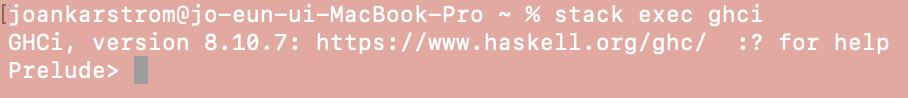
\includegraphics[width=11cm]{STarting.png}
    \caption{Starting GHCI}
    \label{fig:Starting GHCI}
\end{figure}

\medskip\noindent
In this course, we also downloaded and installed BNF Converter, a compiler construction tool that generates a front-end compiler. It allowed us to closely study the grammar of a language and also assist us in creating our own language, which will be explained later in this report.

\subsection{Coding in Haskell}

Haskell is a highly intelligent language; if you were to open the ghci in your terminal, there are a lot of things you could do without even coding an entire .hs file. One can simply type simple math equations into the terminal’s command line it would be able to compute. 

\medskip\noindent
Below is what my terminal looks like when I am testing this. 

\medskip\noindent 
\begin{figure}[htp]
    \centering
    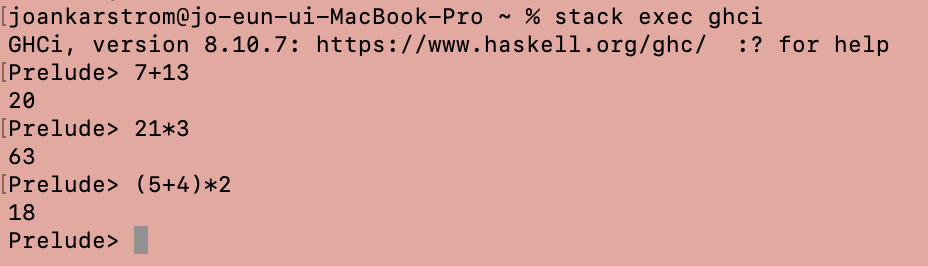
\includegraphics[width=11cm]{TerminalAdd.png}
    \caption{Testing Addition on Terminal using GHCI}
    \label{fig:testing addition}
\end{figure}

\medskip\noindent
Similar to numbers, you can type strings into ghci. Strings are put in double quotes like "this" and can also be added together with ++ to create a larger string.

\medskip\noindent 
\begin{figure}[htp]
    \centering
    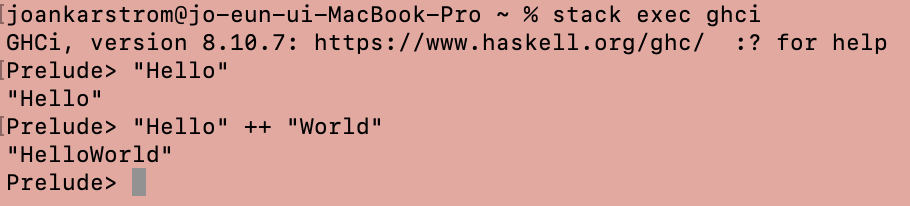
\includegraphics[width=11cm]{TerminalStrings.png}
    \caption{Testing Strings on Terminal using GHCI}
    \label{fig:testing addition}
\end{figure}

\medskip\noindent
One more thing one can do in the ghci terminal is to call functions and write arguments into them. To call a function one write the argument right after the wanted function. 

\medskip\noindent
This how it would look in the terminal. 

\medskip\noindent 
\begin{figure}[htp]
    \centering
    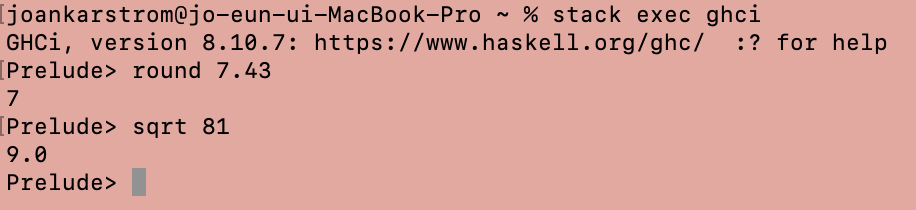
\includegraphics[width=11cm]{TerminalFunction.png}
    \caption{Testing Functions on Terminal using GHCI}
    \label{fig:testing addition}
\end{figure}

\medskip\noindent
Lets move on to coding a Haskell file. The first thing a programmer is taught to code is Hello World. In an .hs file, the first line would look like

\medskip\noindent
\begin{lstlisting}
main = putStrLn "Hello World"
\end{lstlisting}

\medskip\noindent
For Haskell to run, it needs a main function. Building on that, we have the function putStrLn, which takes a string and displays it on the screen instead of print, which calls show on its input first. This takes out "Hello World" and outputs it to the terminal.

\medskip\noindent
Below is what the output looks like using an online Haskell Compiler. 

\medskip\noindent 
\begin{figure}[htp]
    \centering
    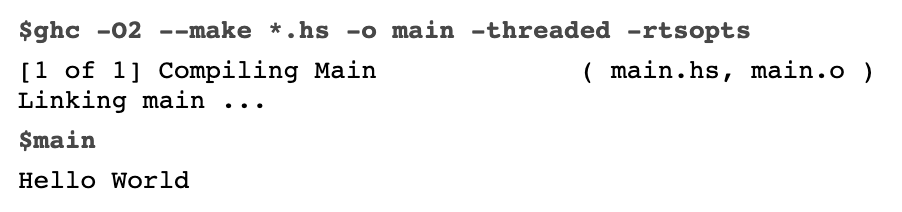
\includegraphics[width=11cm]{OutputHello.png}
    \caption{Hello World output}
    \label{fig:hello world}
\end{figure}

\medskip\noindent
If you were to run this through terminal, you would first compile it in the command line. For this example, let’s assume that the name of our haskell file is test.hs. 

\medskip\noindent
We would write in the terminal to compile

\medskip\noindent
\begin{lstlisting}
ghc test.hs
\end{lstlisting}

\medskip\noindent
Once it has been compiled, you may run it in the terminal by writing

\medskip\noindent
\begin{lstlisting}
./test
\end{lstlisting}

\medskip\noindent
With this, it should create the same output in the terminal as the online compiler as stated above. It is more steps than if you wanted to write something straight into the ghci, but once one creates more significant projects, it is necessary. 

\medskip\noindent
As stated earlier, Haskell is modular, meaning it is a series of functions. So how it tackles functions is a lot different than other languages. To define a function, you must also specify an input and output, which is to be expected, but the way it is written can be confusing. 

\medskip\noindent
For example let’s write a function that takes in two integers and adds them together. 

\medskip\noindent
\begin{lstlisting}
add :: Int -> Int -> Int
\end{lstlisting}

\medskip\noindent
The name of our function, which is what we are trying to have it do is added. The first two Int represents the two arguments that the function is taken. The last Int represents what the function is going to return once it computes. 

\medskip\noindent
The following line would include the actions of the function which in this case would be adding the two inputs together.

\medskip\noindent
\begin{lstlisting}
add :: Int -> Int -> Int
add x y = x + y 
\end{lstlisting}

\medskip\noindent
This function was straightforward as it just took in single variables and returned them.  

\medskip\noindent
Lists are treated a bit differently in Haskell. When declaring a list as an input into a function you must declare the type of list. 

\medskip\noindent
For example this is what the declaration of a function addListLength which takes two lists and brings back an int that is the length of both the lists. 

\medskip\noindent
\begin{lstlisting}
addListLength :: [Int] -> [Int] -> Int
\end{lstlisting}

\medskip\noindent
There are a lot of built in functions that are available but you must remember that Haskell uses recursion in functions. 

\medskip\noindent
Two fast operations used in most functions that parse through a list are "head" and "tail". The reason that these are commonly used is because of their fast run times.

\medskip\noindent
"Head" means getting the first element of the list and "tail" removing the first element in the list. 

\medskip\noindent
Just like earlier how it was discussed how simple functions can be used in the ghci terminal the same is for lists. 

\medskip\noindent
The keyword "let" can be used to name lists and variables alike in the terminal. You can also call them back in the same terminal session. 

\medskip\noindent
This is what it looks like in the terminal if one named and defined a list called test list and called it.

\medskip\noindent 
\begin{figure}[htp]
    \centering
    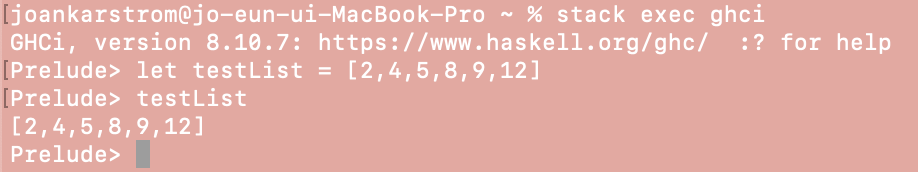
\includegraphics[width=11cm]{NameLists.png}
    \caption{Naming Lists on Terminal using GHCI}
    \label{fig:naming lists}
\end{figure}

\medskip\noindent
You can also add lists together just like integers and strings. The list being added will be added behind the original list.

\medskip\noindent 
\begin{figure}[htp]
    \centering
    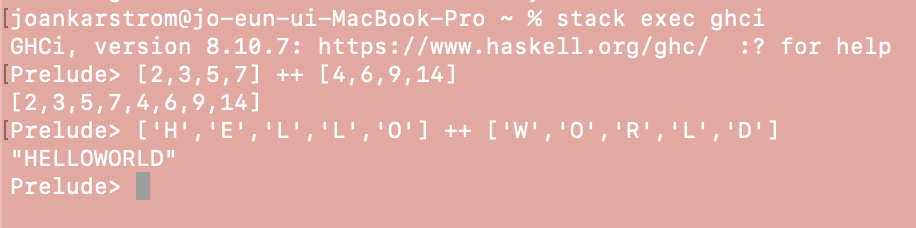
\includegraphics[width=11cm]{NamingLists.png}
    \caption{Adding Lists on Terminal using GHCI}
    \label{fig:adding lists}
\end{figure}

\medskip\noindent
This "++" adds the two lists together although it does not sort them, and it just adds the second list to the first one. 

\medskip\noindent
The second input in the command line shows a list of char's being added together to say "HelloWorld.” 

\medskip\noindent
When a programmer thinks of a list they would default thinking of a list to look like this.

\medskip\noindent
\begin{lstlisting}
[1,2,3,4]
\end{lstlisting}

\medskip\noindent
In Haskell they are treated and look like this.

\medskip\noindent
\begin{lstlisting}
1:2:3:4:[]
\end{lstlisting}

\medskip\noindent 
\begin{figure}[htp]
    \centering
    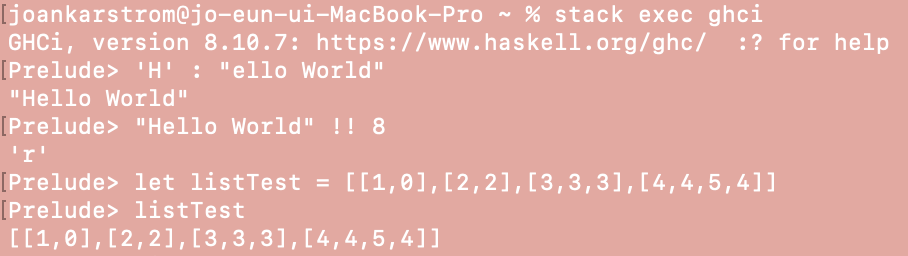
\includegraphics[width=11cm]{AppendingLists.png}
    \caption{Appending Lists on Terminal using GHCI}
    \label{fig:Appending lists}
\end{figure}

\medskip\noindent
More things that are shown above is how variables can be added to lists using ':'. Using '!!' the variable at a certain spot. Lastly, lists can also hold lists, and they don't have to be the same size to be in the same list.

\subsection{Lazy vs. Non-Strict Programming}

One of the biggest things That Haskell is often described as is "Lazy," but it is not necessarily "lazy". Technically Haskell is non-strict. Haskell is one of the very few functional programming languages that default to a “lazy” way of evaluating, while other languages have this option but are not widely used. 

\medskip\noindent
Lazy is a charming way of saying that the compiler waits and procrastinates to evaluate the expression \cite{LP}. This means that specific values or projects are not considered until they are called upon or used. 

\medskip\noindent
Strict evaluation is used in almost every other language, which means that it is computed even if the expression is not needed. 

\medskip\noindent
Non-Strict in an algebraic sense, when you are assessing an argument, it works from the outside in, not the other way around. \cite{NS} 

\medskip\noindent
In math, we are taught to work our way out as it is how to evaluate expressions using order of operations or “P. (parentheses) E. (exponents) M. (multiplication) D. (division) A. (addition) S. (subtraction).” 

\medskip\noindent
Lets take the equation $$(a + (b - c))$$ 
First, we are going to evaluate this as we would in math class. 
Parentheses are first, which means we must complete what is in the innermost parentheses first so that we would calculate the expression $$(b - c)$$. For the sake of this example, we will say “b - c = d.” So the equation would now look like $$(a + (d))$$ Since we have completed everything in the parenthesis, we can now add d to a, which would give us our final answer. 

\medskip\noindent
How lets compare this to what we would see in Haskell. $$(a + (b - c))$$

\medskip\noindent
In the non-strict schematic, an expression can have value even if some of its subexpressions do not. 

\medskip\noindent
In Haskell, you would first reduce the "+" and then you would reduce the inner $$(b - c)$$ Now, as you can see, it works almost the complete opposite.

\medskip\noindent
The reason that Haskell is "non-strict" is because of how it is used to evaluate expressions. Let's say you have an expression that evaluates to "bottom"; has an infinite loop or error; if you were a programming language that worked in to out, you would always find that "bottom" but because Haskell or a "Non-Strict" language works out to in some of these are not evaluated. \cite{LNS}

\medskip\noindent
Though some people use it interchangeably, "Lazy" and "Non-Strict" do not mean the same thing as similar as they are. 

\medskip\noindent
For example, Haskell has some cases where it is not lazy at all, for instance, pattern matching. You can make this lazy but usually not in practice, since you are actively looking for matches. 

\subsection{Recursive}

\medskip\noindent
Recursion is most commonly used when talking about mathematics and means "the repeated application of a recursive procedure or definition." \cite{RR} 

\medskip\noindent
In programming case its definition is "a computer programming technique involving the use of a procedure, subroutine, function, or algorithm that calls itself one or more times until a specified condition is met at which time the rest of each repetition is processed from the last one called to the first", basically it is used to describe a function that calls upon its self. 

\medskip\noindent
Haskell is a perfect language to write recursive expressions and is sometimes the only way to write them. This is because there is no such thing as while loops or for loops in this language, which seems weird because we use these things all the time when programming. 

\medskip\noindent
The most common example of recursion is factorial. 

\medskip\noindent
In Haskell, this is what that function would look.

\medskip\noindent
\begin{lstlisting}
fact :: Int -> Int 
fact 0 = 1 
fact n = n * fact ( n - 1 )  
\end{lstlisting}

\medskip\noindent
To show this, we are going to write a minimum function \cite{MF} in Haskell. We will have it take in a list of things assuming that it can be ordered (using the Ord class) and return the lowest value.

\medskip\noindent
First, we are going to start by importing the list.

\medskip\noindent
\begin{lstlisting}
minimum' :: (Ord a) => [a] -> a  
\end{lstlisting}

\medskip\noindent
In this next part, we must take in account if an empty list is passed, so we take the empty value minimum'[] and we return the error "minimum of empty list". 

\medskip\noindent
The next thing we write is telling the program if there is only one value in a list, return that value since that would be the minimum number in that list!

\medskip\noindent
\begin{lstlisting}
minimum' :: (Ord a) => [a] -> a  
minimum' [] = error "minimum of empty list"  
minimum' [x] = x  
\end{lstlisting}

\medskip\noindent
Now its time to implement the function that minimum will execute. So in this function, if the value that is passed through is less than the minimum, then x will be the new minimum; if not, then "cur" will be the minimum value. 

\medskip\noindent
\begin{lstlisting}
minimum' (x:xs)   
    | x < min = x  
    | cur = min  
    where min = minimum' xs
\end{lstlisting}

\medskip\noindent
Putting this all together, we would have the function: \cite{MF}

\medskip\noindent
\begin{lstlisting}
-- run the transition function on a word and a state
minimum' :: (Ord a) => [a] -> a  
minimum' [] = error "minimum of empty list"  
minimum' [x] = x  
minimum' (x:xs)   
    | x < min = x  
    | cur = min
    where min = minimum' xs
\end{lstlisting}

\medskip\noindent
Now, this was a great example of how to use recursion to "loop" through information whereas in python or Java, one would just use a while for if then else function.

\subsection{Python V. Haskell}

At Chapman, the first computer science class that you take is taught in Python. In my opinion, I believe Python is one of the easiest programming languages to learn and is a great way to start introducing new learners of coding to logic. 

\medskip\noindent
Python, visually, is straightforward to read, for example unlike Java which requires methods and functions to be enclosed with “{ }” and almost every line requires a “;” at the end.

\medskip\noindent
For example, let’s take a look at the bubble sorting algorithm in Python and in Haskell. Before we dive into the algorithm, let’s explain what the bubble sorting algorithm is. It is a sorting algorithm that swaps adjacent numbers if they are in the wrong order \cite{BSS}. 

\medskip\noindent
First, let’s take a look at the python version of the bubble sorting algorithm.

\medskip\noindent
\begin{lstlisting}
def bubbleSort(arr):
    n = len(arr)
 
    for i in range(n):
        for j in range(0, n-i-1):
            if arr[j] > arr[j+1] :
                arr[j], arr[j+1] = arr[j+1], arr[j]
 
# code to test above
arr = [32, 54, 44, 23, 29, 49, 63]
 
bubbleSort(arr)
print ("Sorted array is:")
for i in range(len(arr)):
    print ("%d" %arr[i]), 
\end{lstlisting}
\cite{BSP}

\medskip\noindent
We can break this down line for line. It starts off with defining the method and getting the length of the array setting it to n. They then have 2 for loops that loop through the array and then slowly sort through. 

\medskip\noindent
While it loops through the array it looks at the current spot compared to the number to the right and if that number is bigger or smaller, the number is moved respectfully. 

\medskip\noindent
Now lets look at the bubble sort algorithm in Haskell. 

\medskip\noindent
\begin{lstlisting}
bSort [] = []
bSort x = case new == x of
               True -> x
               False -> bSort new
    where
        new = bSortInner x

        bSortInner [] = []  
        bSortInner [x] = [x]
        bSortInner (x : y : xs)
            | y <= x = y : bSortInner (x : xs)
            | otherwise = x : bSortInner (y : xs)
\end{lstlisting}
\cite{BSH}

\medskip\noindent
We first start with our type signature in this case is bSort (bubble sort). It takes in a list and returns the list sorted (Assuming that the list is orderable). From there we take our base case which is an empty list and the next case is our exit condition. 

\medskip\noindent
bSortInner does the work in this sort algorithm, once we have simplified it down to one single case we can implement the sorting part. 

\medskip\noindent
We now have two inner cases. 

\medskip\noindent
\begin{lstlisting}
y <= x 
y > x
\end{lstlisting}

\medskip\noindent
That is organized into the code along with the otherwise piece of the code.

\medskip\noindent
Both of these are the bubble sorting algorithm but they are implemented in different ways due to the different programming languages. Not only that but because of how the languages are built. 

\medskip\noindent
In the next section of this report more will be said about the grammar of programs and how because they differ they also act differently.

\section{Programming Languages Theory}

\medskip\noindent
In this course we have gone over multiple theories and how they pertain to programming languages. 

\medskip\noindent
Specifically we have spent a decent amount of time learning lambda calculus and how to evaluate functions with it. 

\medskip\noindent
Although I will probably never try and build a programming language from scratch, it is still very beneficial to learn the logic on how grammar is used in the language and helps bring another layer of understanding behind choosing a language to program in.

\subsection{Parsing}

\medskip\noindent
The definition of parsing is "analyze (a string or text) into logical syntactic components, typically in order to test conform-ability to a logical grammar."\cite{PAR} During the programming languages class we have talked about grammar as it being a way people literally create and build programming languages. 

\medskip\noindent
In English we use grammar to create sentences with meaning. We have nouns, verbs, adjectives ect. to better explain to others what we are trying to say. With better communication, the faster and more efficient work can be done. 

\medskip\noindent
It is the same in programming languages. Different languages have different syntax or ways to write similar things and parsing taking the grammar to read a language. 

\medskip\noindent
The most popular languages that programmers use when assigning a variable use "=" as opposed to ":=" in languages such as Ada or Maple, or even "def" in Postscript. Although this is more of a syntax opinion than a grammar. 

\medskip\noindent
\begin{lstlisting}
minimum' :: (Ord a) => [a] -> a  
\end{lstlisting}

\medskip\noindent
The grammar is the building blocks of a language and can determine the limitations of that language or the weaknesses of it. What parsing does is it reads a grammar file looking for patterns. 

\medskip\noindent
It reads word for word looking at what is a variable and what is an expression and what the relationship between the two are. 

\medskip\noindent
Earlier in this report I compared Haskell to Python the programming language. Every programming language has a grammar to it but it is not necessary to parse it as the most popular languages have emulator such as docker to run the languages.

\medskip\noindent
The grammar used in this class was not too difficult or big so it took a small amount of time to run and generate a parser but that is not the case with every language.

\medskip\noindent
Below is a segment from Python's documented grammar.

\medskip\noindent
\begin{lstlisting}
assignment:
    | NAME ':' expression ['=' annotated_rhs ] 
    | ('(' single_target ')' 
         | single_subscript_attribute_target) ':' expression ['=' annotated_rhs ] 
    | (star_targets '=' )+ (yield_expr | star_expressions) !'=' [TYPE_COMMENT] 
    | single_target augassign ~ (yield_expr | star_expressions) 
augassign:
    | '+=' 
    | '-=' 
    | '*=' 
    | '@=' 
    | '/=' 
    | '%=' 
    | '&=' 
    | '|=' 
    | '^=' 
    | '<<=' 
    | '>>=' 
    | '**=' 
    | '//=' 

global_stmt: 'global' ','.NAME+ 
nonlocal_stmt: 'nonlocal' ','.NAME+ 
\end{lstlisting}
\cite{PYT} 

\medskip\noindent
As you can see above, this portion of the code is defining assignments. The actual grammar file is a lot bigger and can be seen at the sited website.  

\medskip\noindent
Python is not the only language that has this, as stated before, every programming language has some sort of grammar.

\medskip\noindent
Listed below are some quick links pertaining to the grammar of some of the most popular programming language's grammar.

\begin{enumerate}
  \item \href{http://www.csci.csusb.edu/dick/samples/java.syntax.html}{Java's Grammar} 
  \item \href{https://medium.com/@mujjingun_23509/full-proof-that-c-grammar-is-undecidable-34e22dd8b664}{Full Proof that C++ Grammar is Undecidable} 
  \item \href{https://docs.microsoft.com/en-us/dotnet/csharp/language-reference/language-specification/lexical-structure}{Lexical structure of C sharp} 
\end{enumerate}

\subsection{Grammar}

\medskip\noindent
As Grammar makes up the foundation of a language, there are two ways that one's grammar could be defined as "ambiguous" or "Non-ambiguous". 

\medskip\noindent
Ambiguous or "Context Free" grammar is grammar that when an input has multiple trees. When first learning about Haskell one learns how the language reads a statement and how it takes that apart. A tree is a visual way to break down the variables and arguments in the way that the program will read it. 

\medskip\noindent
In the example of ambiguous grammar when a tree is created, there are actually two trees that are created. One reading the input from left to right and the other one being read from right to left. 

\medskip\noindent
Below this is how the trees will look like if we were evaluating the expressions $$2+3+4$$ In my tree I define the mathematics function being applied and the type of variable that is being affected. 

\medskip\noindent 
\begin{figure}[htp]
    \centering
    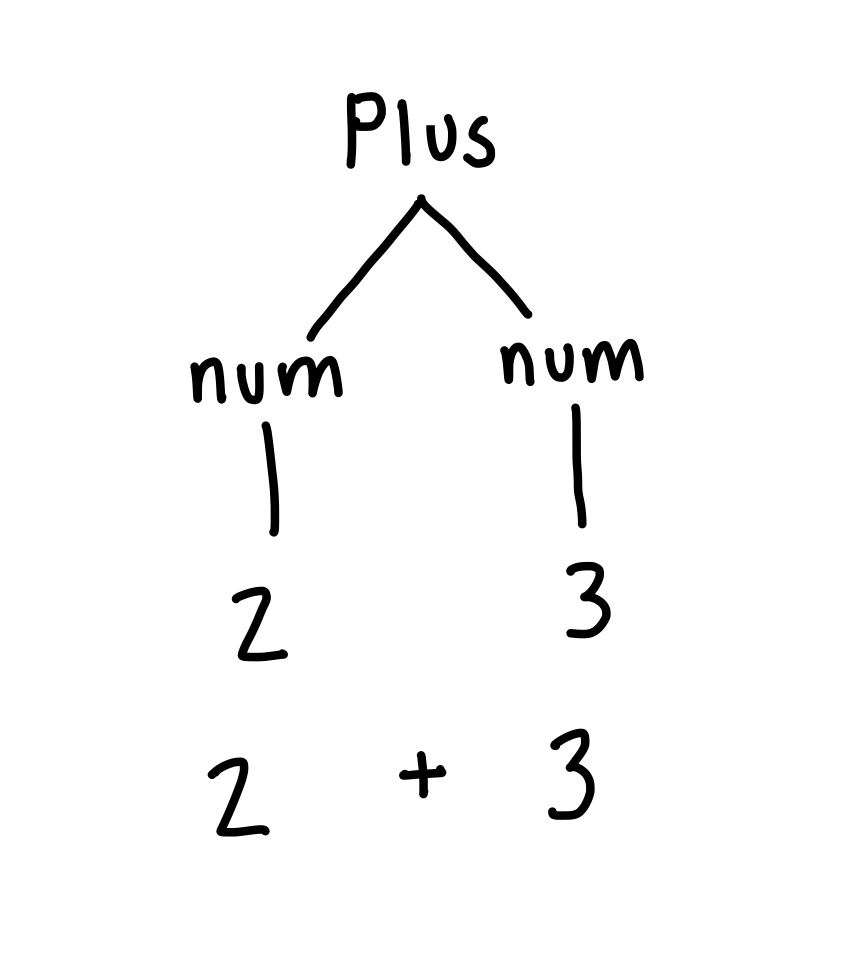
\includegraphics[width=7cm]{2+3tree.jpg}
    \caption{2+3+4 Ambiguous Parsing Tree}
    \label{fig:Parsing Tree 1}
\end{figure}

\medskip\noindent
On the bottom of each tree you can see that when you read down the tree, they are the same expression that both output a 9 but the trees look different. The part that makes this grammar ambiguous is that using the same grammar rules there were 2 different trees that were produced. 

\medskip\noindent
This is a very simple example but it could become a lot more complicated when you add multiple math expressions and different parenthesis. Below is an example of grammar that is "non-ambiguous". ** Not correct image right now

\medskip\noindent 
\begin{figure}[htp]
    \centering
    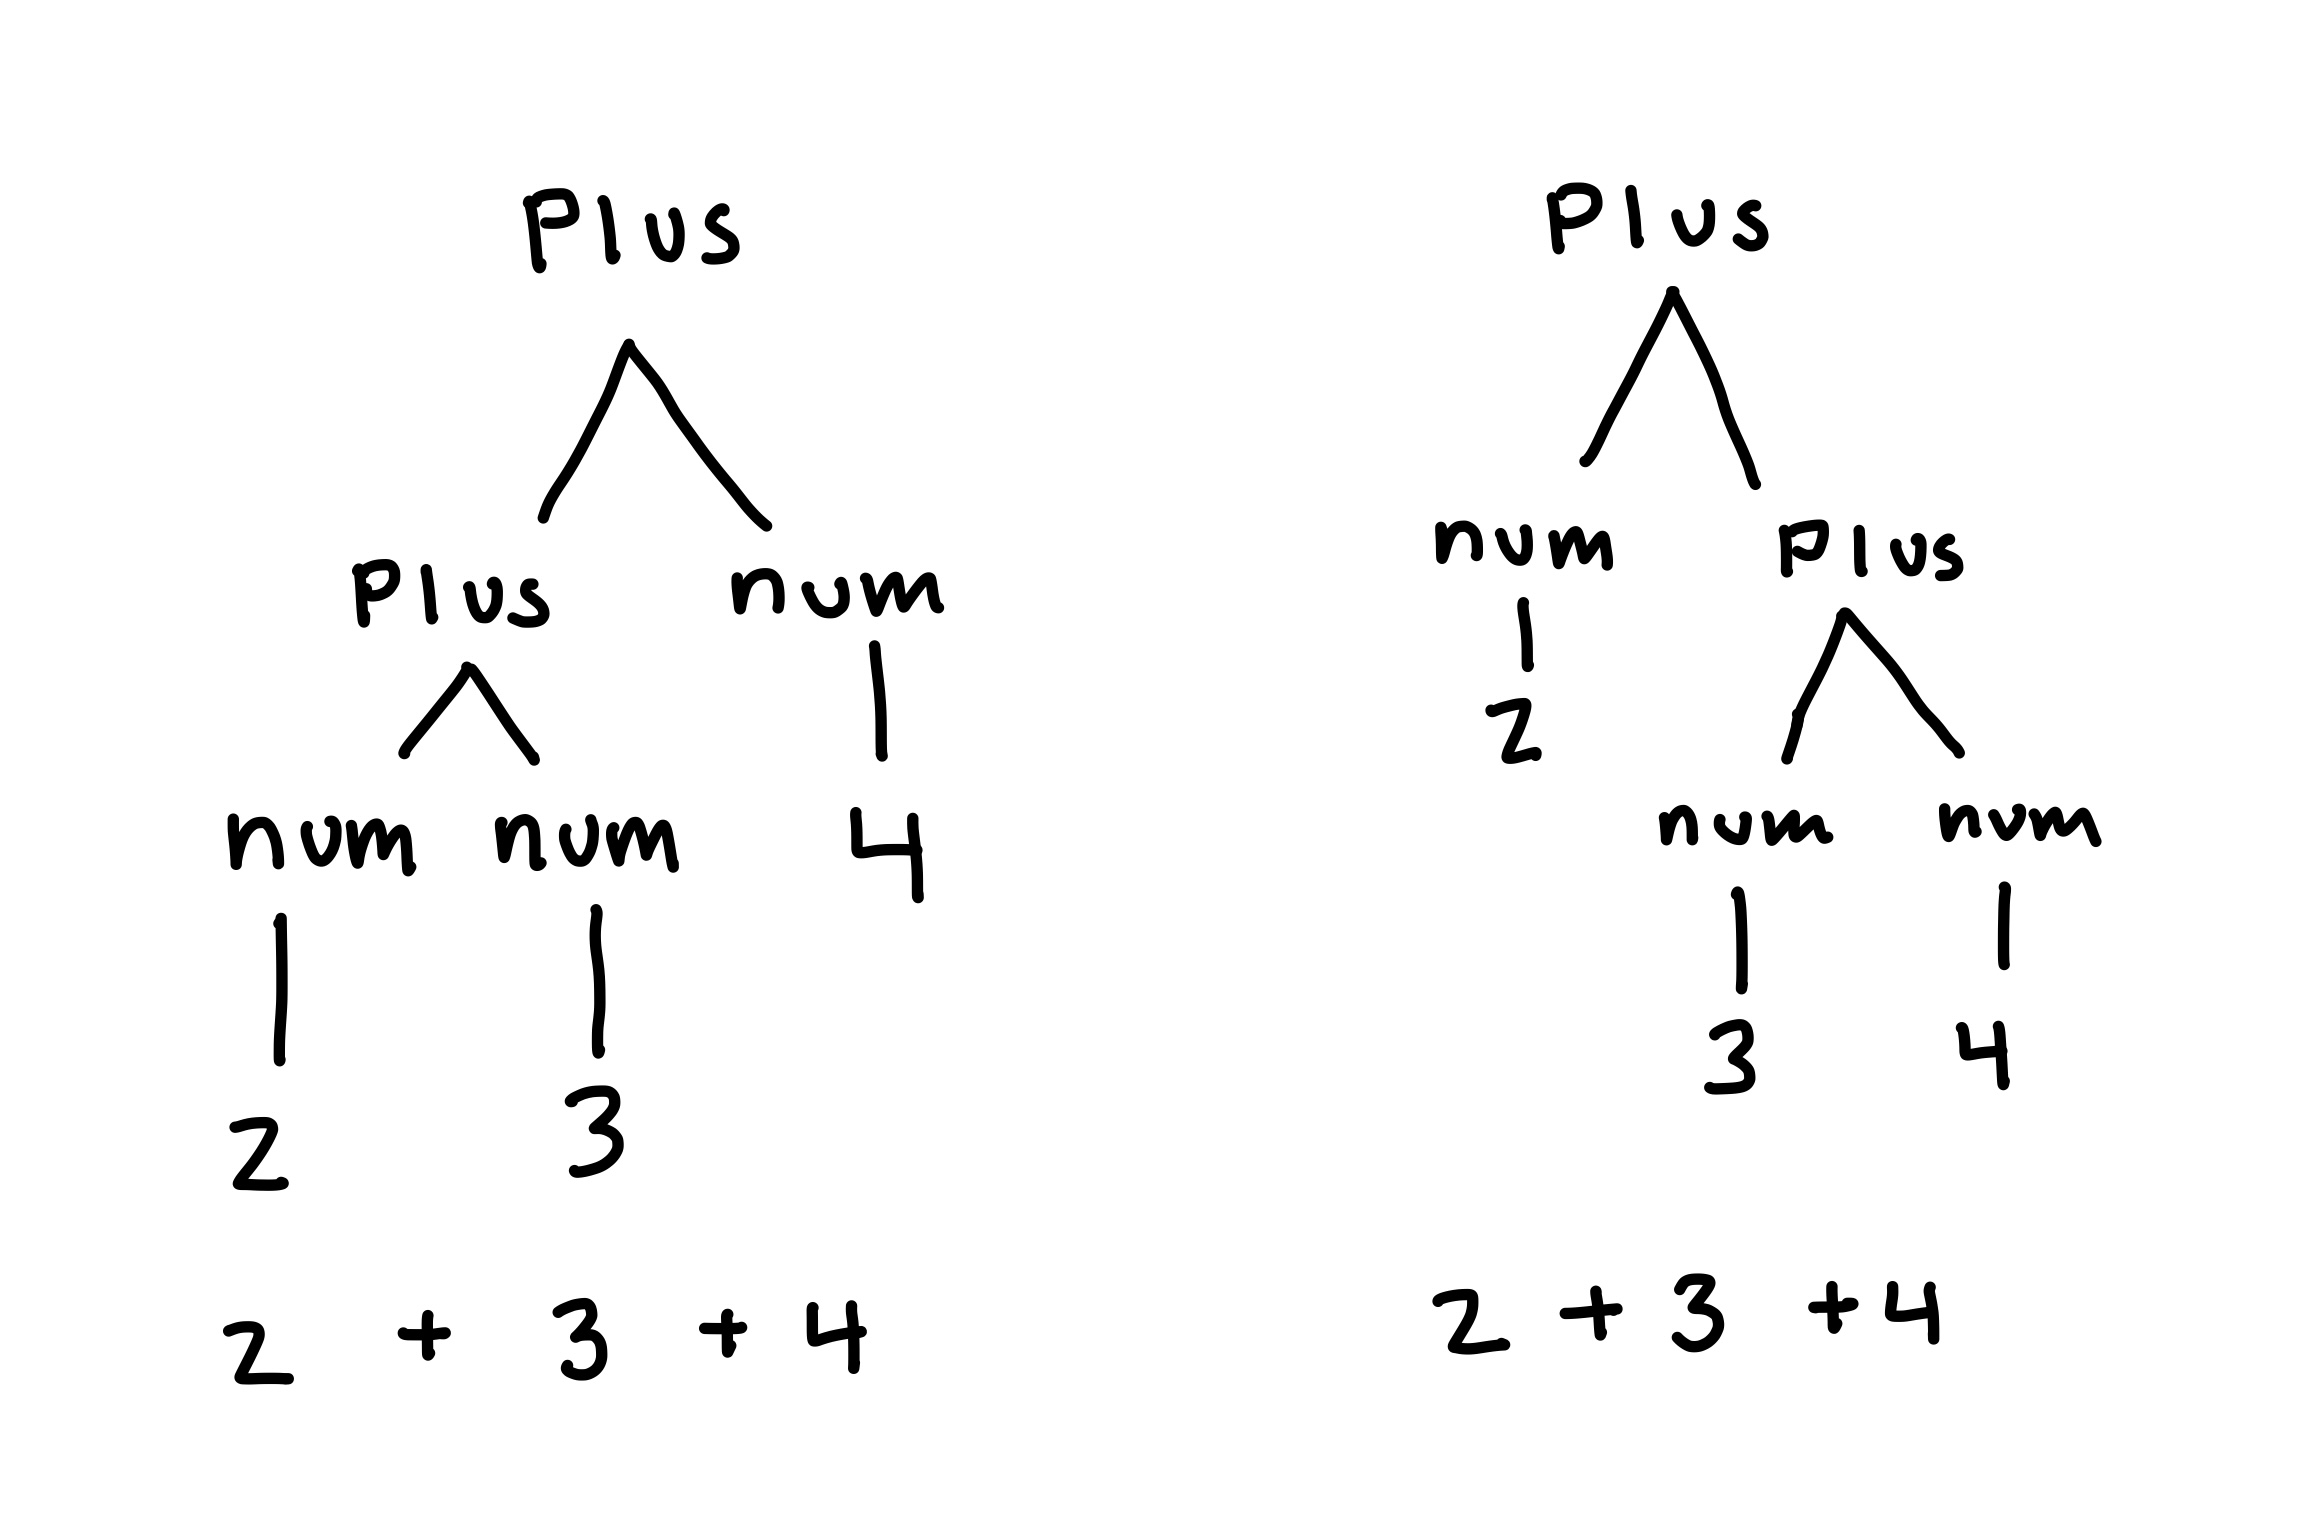
\includegraphics[width=10cm]{IMG_0653.jpg}
    \caption{ Non-Ambiguous Parsing Tree}
    \label{fig:Parsing Tree 2}
\end{figure}

\medskip\noindent
I think it is very important that the trait of ambiguity does not have to do with the language, its all to do with the grammar of the language. 

\medskip\noindent
There is not a set way to get rid of the ambiguity, instead you must go through the grammar expression by expression and double check there is only one way to do it according to the definitions that have been set.\cite{AG} 

\medskip\noindent
Although it is troublesome to do, trees are a very simple way of checking this and it is easier to read then the actual coded grammar itself.

\medskip\noindent
Lets make our first expression that we worked with non-ambiguous. This is a very simple expression and takes a very simple fix for it to only create one tree and that is parentheses. 

\medskip\noindent
I explained earlier in my paper about in math P.E.M.D.A.S. is very practical to helping solve logistic issues in computing as it has the same theory. 

\medskip\noindent
Below is the tree that would be if we changed 2+3+4 to (2+3)+4

\medskip\noindent 
\begin{figure}[htp]
    \centering
    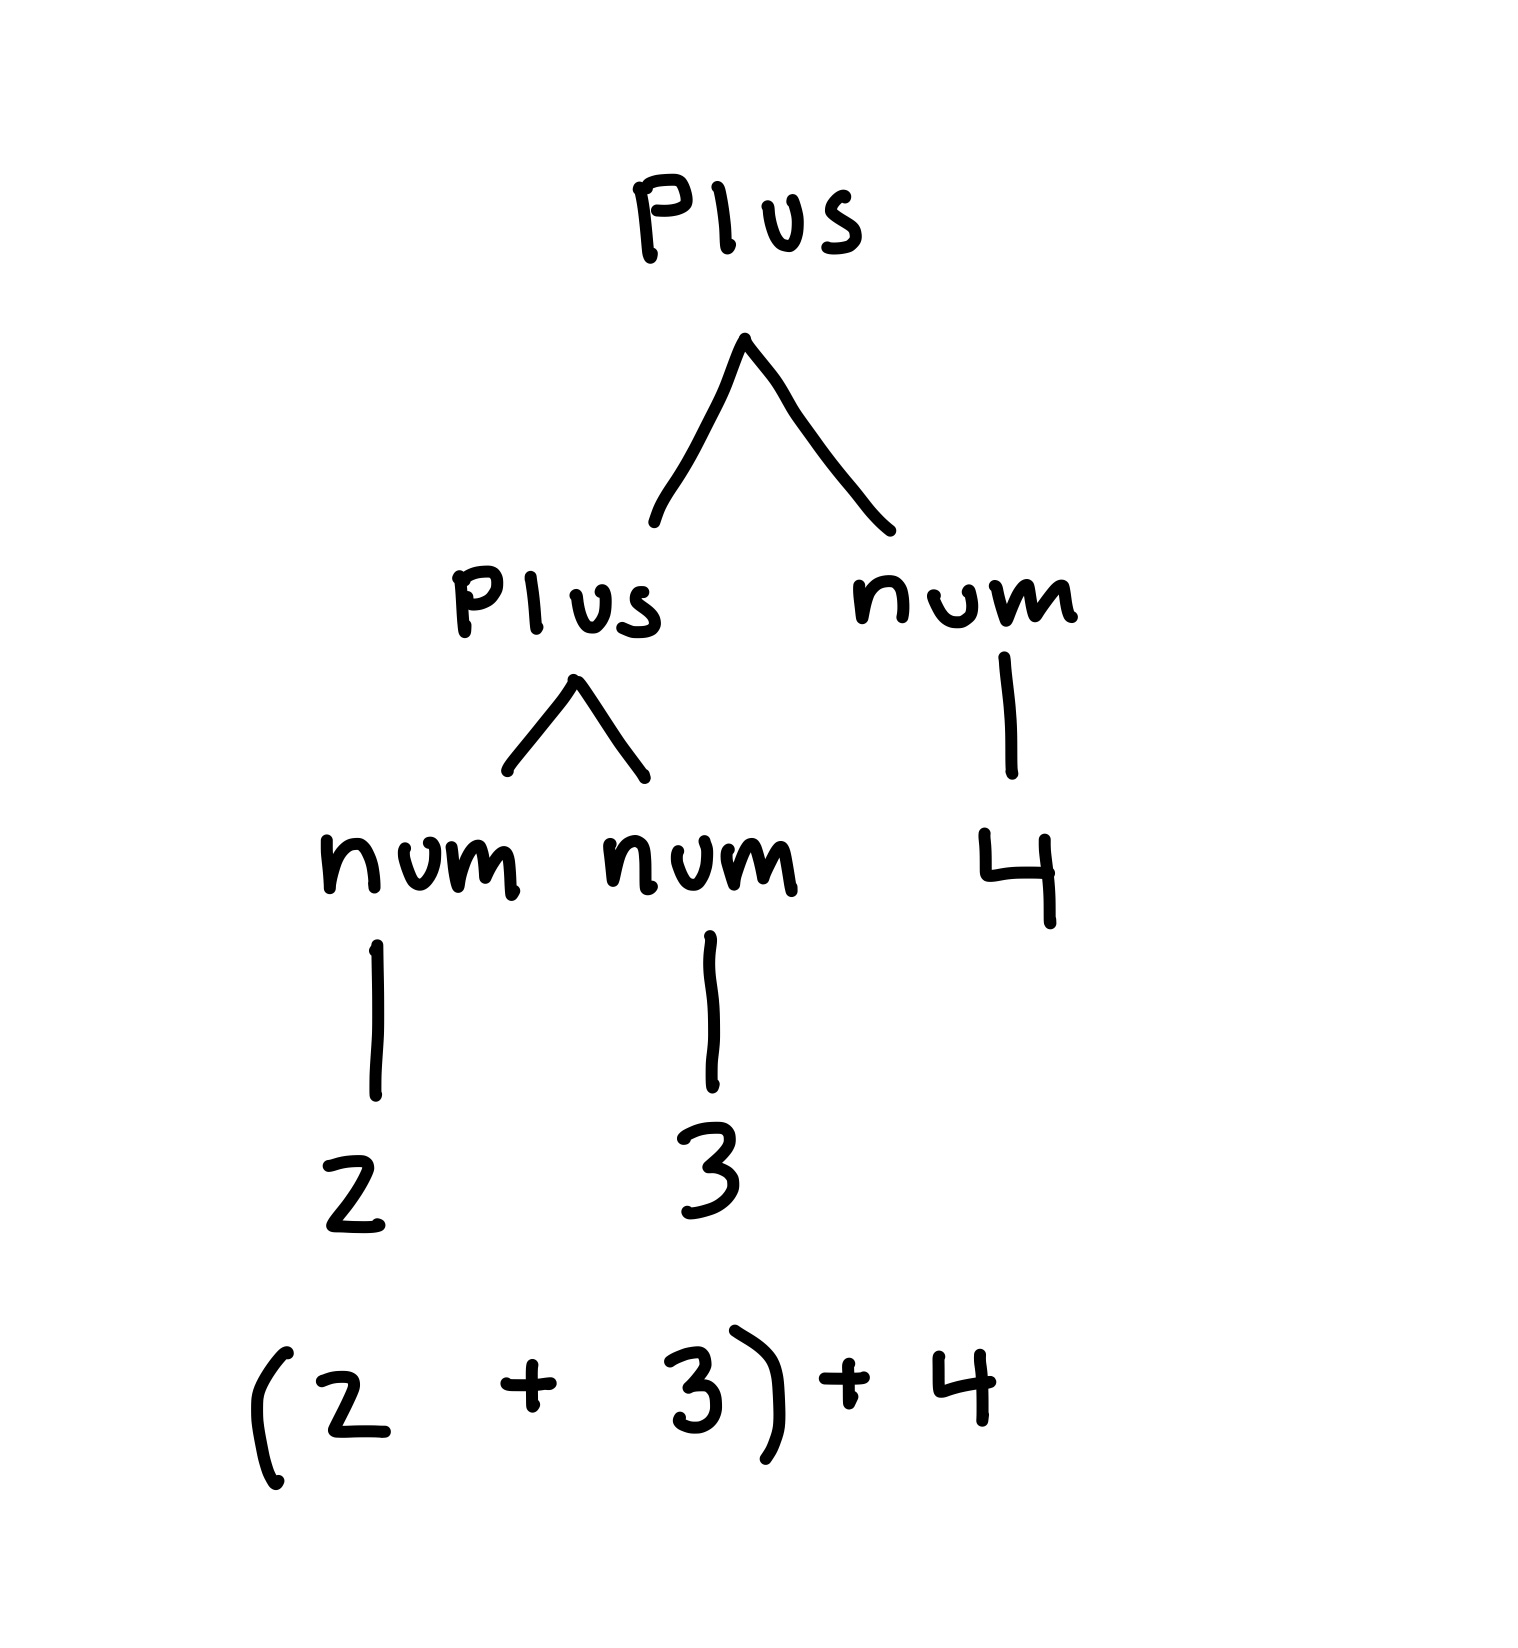
\includegraphics[width=7cm]{IMG_0654.jpg}
    \caption{2+3+4 (Un)Ambiguous Parsing Tree}
    \label{fig:Parsing Tree 3}
\end{figure}

\medskip\noindent 
As you can see the tree looks very similar to the left tree in our first example as its reading left to right like in normal math. In this tree, the expression in the parenthesis is further defines lower in the tree and just like the earlier example the output is 9. 

\medskip\noindent
The right tree from the first example would not work as you must keep the parenthesis together. 

\subsection{Lambda Calculus}

Lambda Calculus is " a simple notation for functions and application. The main ideas are applying a function to an argument and forming functions by abstraction."\cite{LA} Earlier when the history of Haskell was discussed, LISP was mentioned. Lambda Calculus was the basis of this language. 

\medskip\noindent
A lot of what we did with Lambda Calculus was translating this mathematical language into code and computing it as it is not a common language to compute in.

\medskip\noindent
To better understand Lambda Calculus, I will discuss a few examples. First is pure lambda calculus. 
$$ (\lambda x.x)y$$

\medskip\noindent
This would be simplified down to just.
$$y$$

\medskip\noindent
The next example is a plus one function, it is not pure lambda as it includes a plus sign.
$$ \lambda x.x+1$$

\medskip\noindent
To break this down this function has one parameter which is 'x' and the body of the function is 'x+1'.

\medskip\noindent
This is technically not a pure lambda function as it has a + sign. 

\medskip\noindent
We can expand on this example and use this function! Lets run 2 through this and to do that we would add it at the end of the expression. In lambda equal signs are rarely used so adding the 2 on the end is sufficient enough to understand you are plugging in 2 for this function.
$$ (\lambda x.x+1)2$$

\medskip\noindent
Just looking at this would be a bit difficult so we can draw a parse tree to break down what exactly this function is trying to say.

\medskip\noindent 
\begin{figure}[htp]
    \centering
    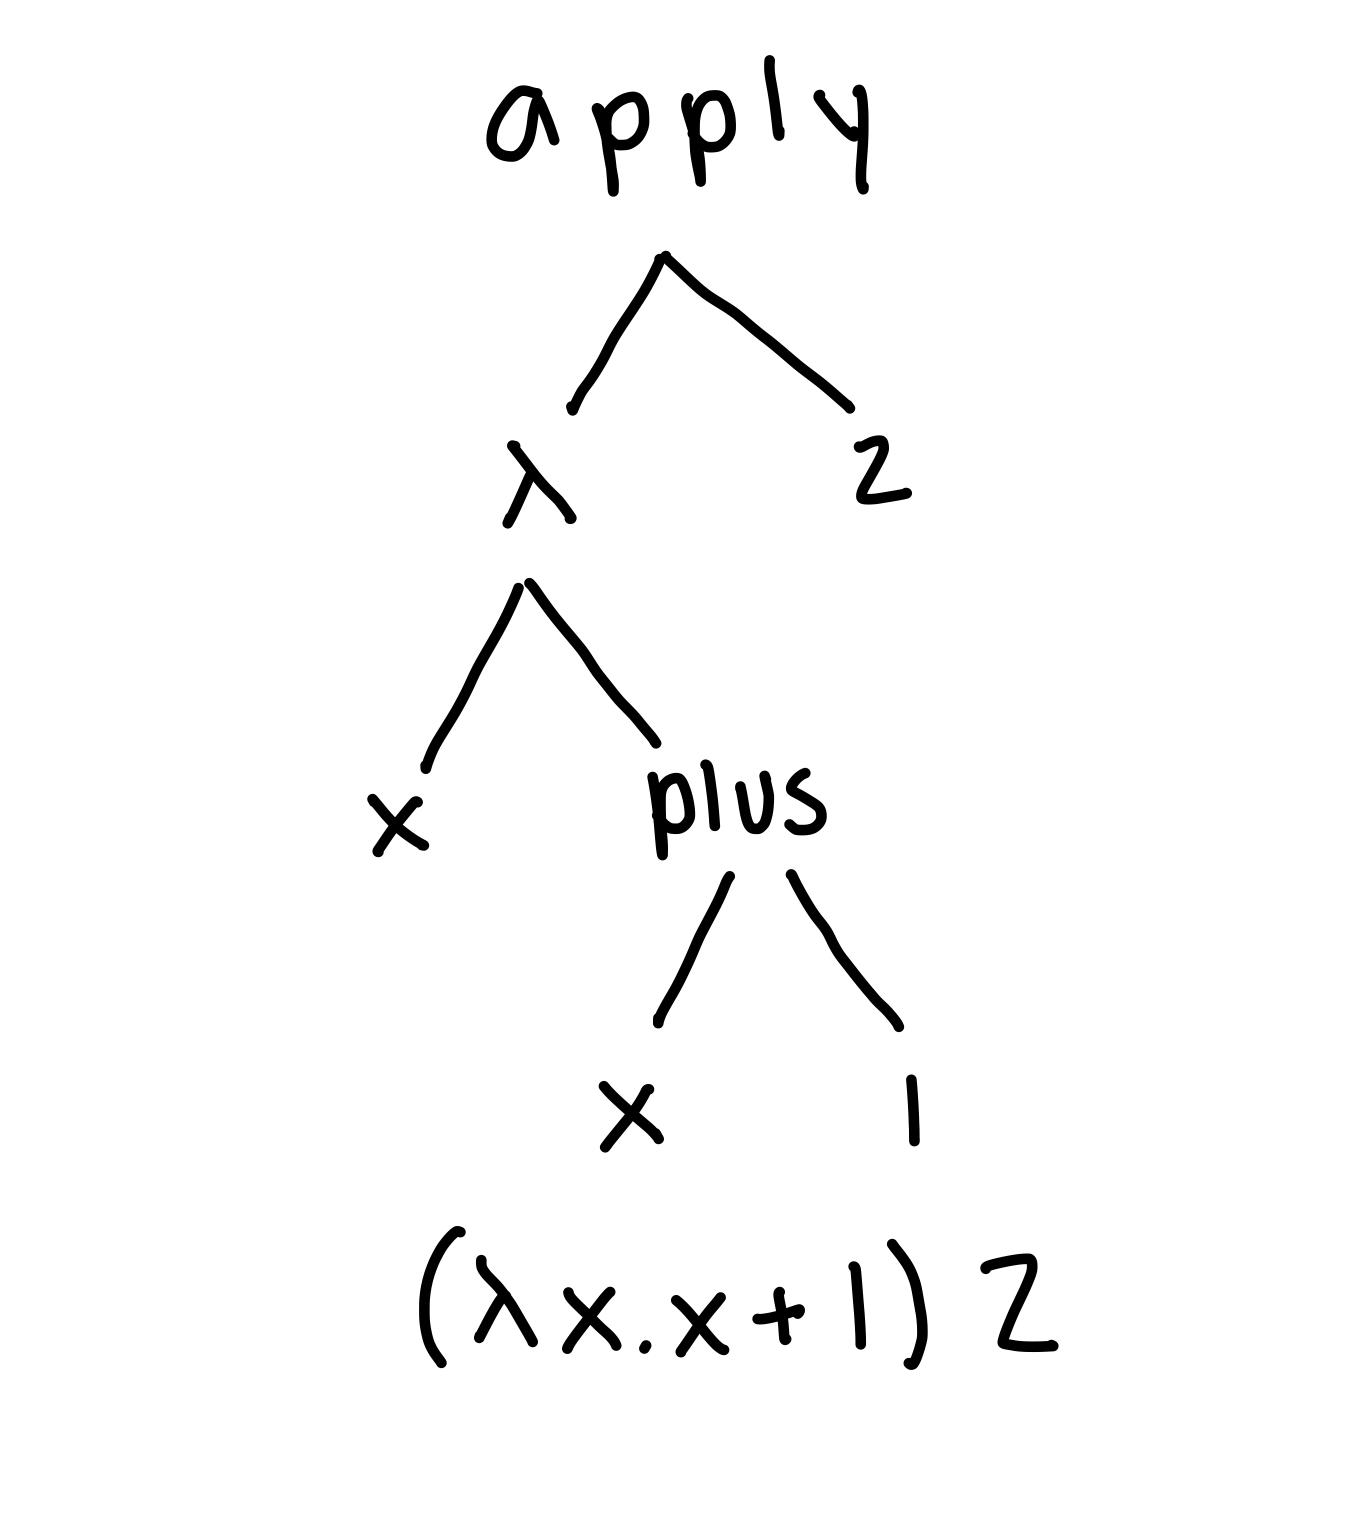
\includegraphics[width=7cm]{lambdaExample1.jpg}
    \caption{Lambda Example 1 Tree}
    \label{fig:Lambda Example Tree}
\end{figure}

\medskip\noindent
Earlier we went over order of operations in parsing trees and you can see how in this example how high up lambda is on this tree. If we use the rule that we learned earlier we know that lambda is taking in expressions to evaluate so if we want to get the answer to this function we would need to simplify things down.

\medskip\noindent
If we were to simplify this tree to get out it would look like.

\medskip\noindent 
\begin{figure}[htp]
    \centering
    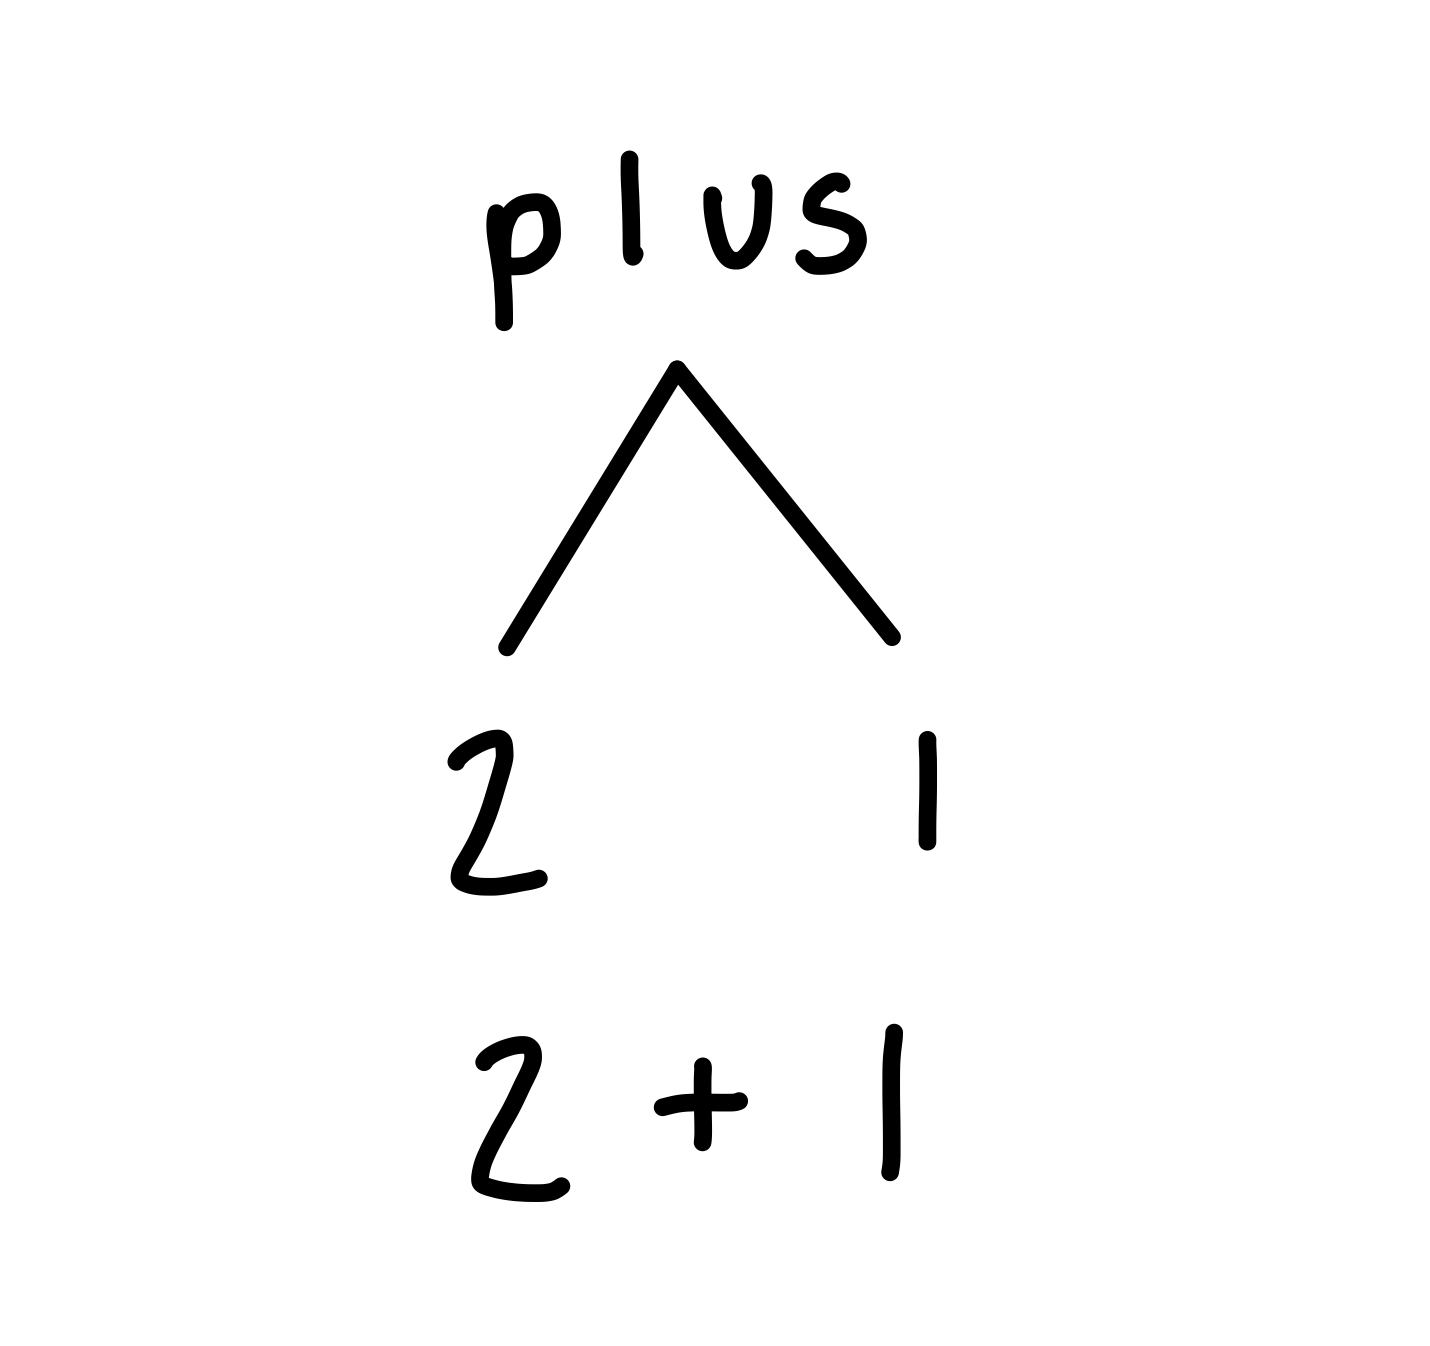
\includegraphics[width=6cm]{IMG_0676.jpg}
    \caption{Lambda Example 1 Simplified Tree}
    \label{fig:Lambda Example Tree Simplified}
\end{figure}

\medskip\noindent
Now this is exactly what output was wanted from this function, since it is a plus one function we would want whatever number was inputted to the function to be one higher which in this case would be 2+1=3.

\medskip\noindent
That was a super simple example but lets do something more complicated with two different functions.
$$ (\lambda x.x+4)(\lambda y.y+3)2$$

\medskip\noindent
Just like last time, lets create a tree that would better help us understand what the function is asking us to do. 

\medskip\noindent 
\begin{figure}[htp]
    \centering
    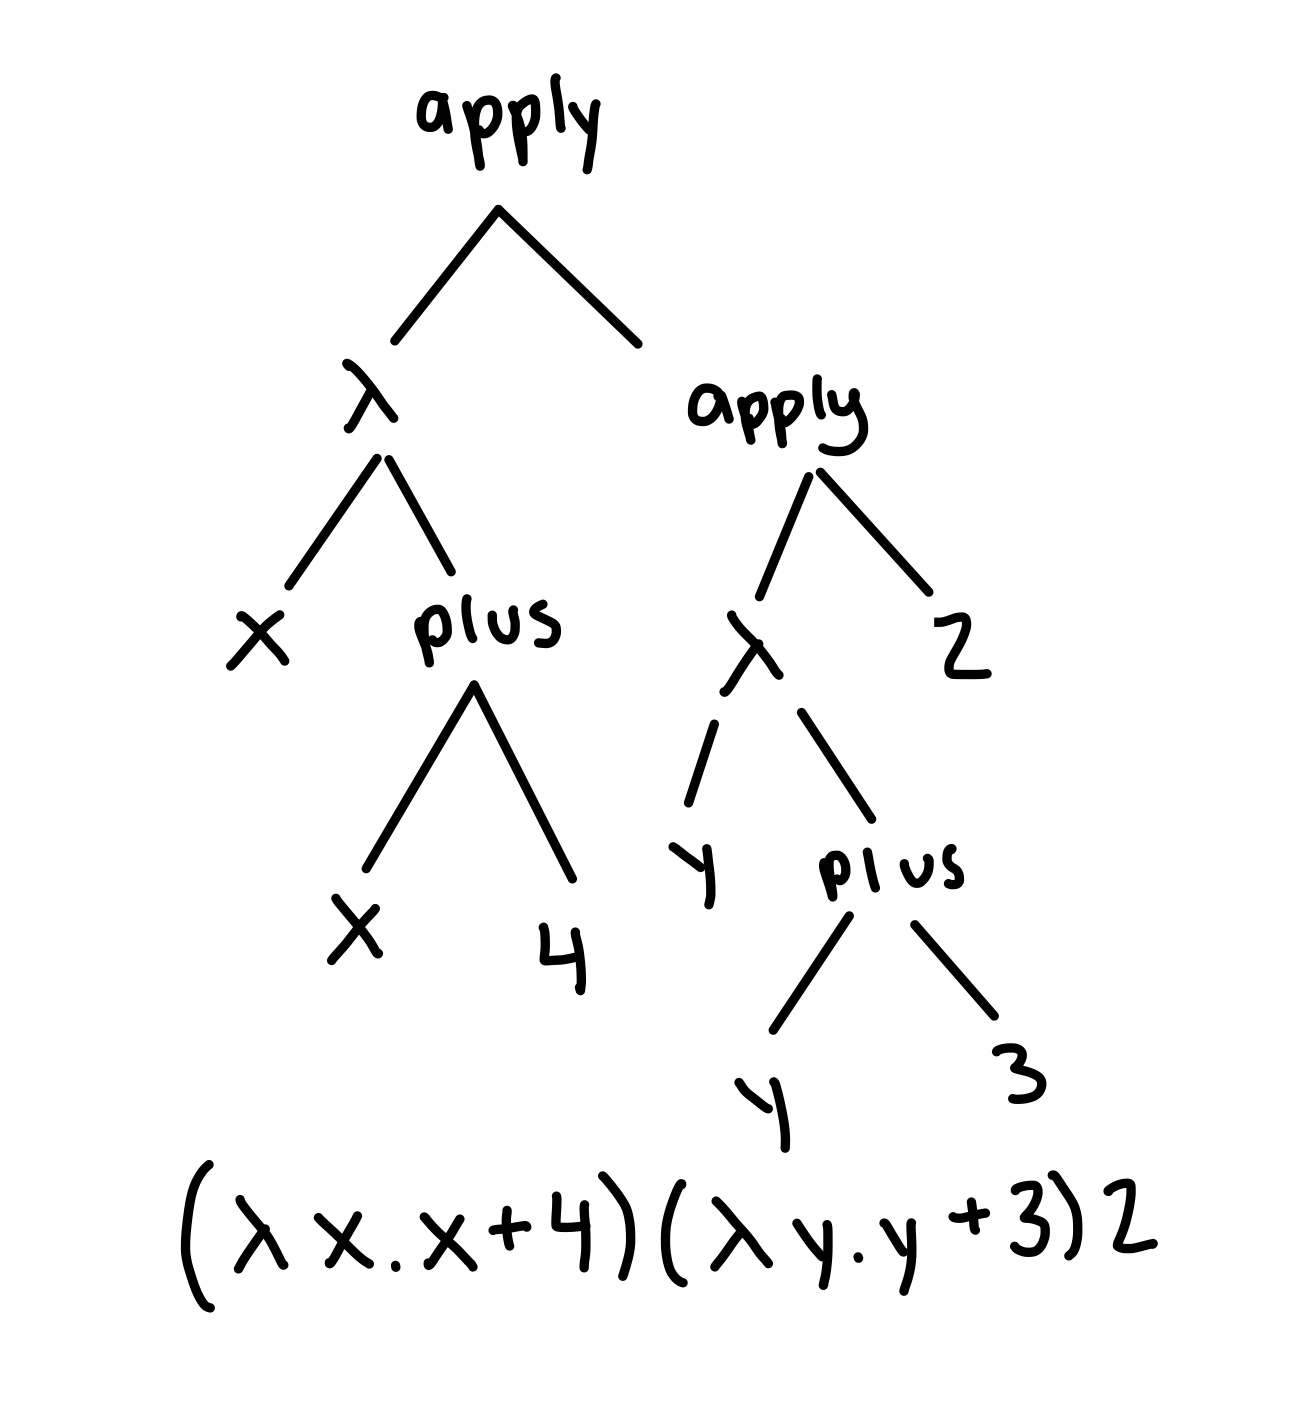
\includegraphics[width=7cm]{LambdaEx2.jpg}
    \caption{Lambda Example 2}
    \label{fig:Lambda Example 2}
\end{figure}
\cite{LFG}

\medskip\noindent
The final equations that we would get from this would be $$2+3+4$$ Below is what the parsing tree would look like once we start to simplify the process. 

\medskip\noindent 
\begin{figure}[htp]
    \centering
    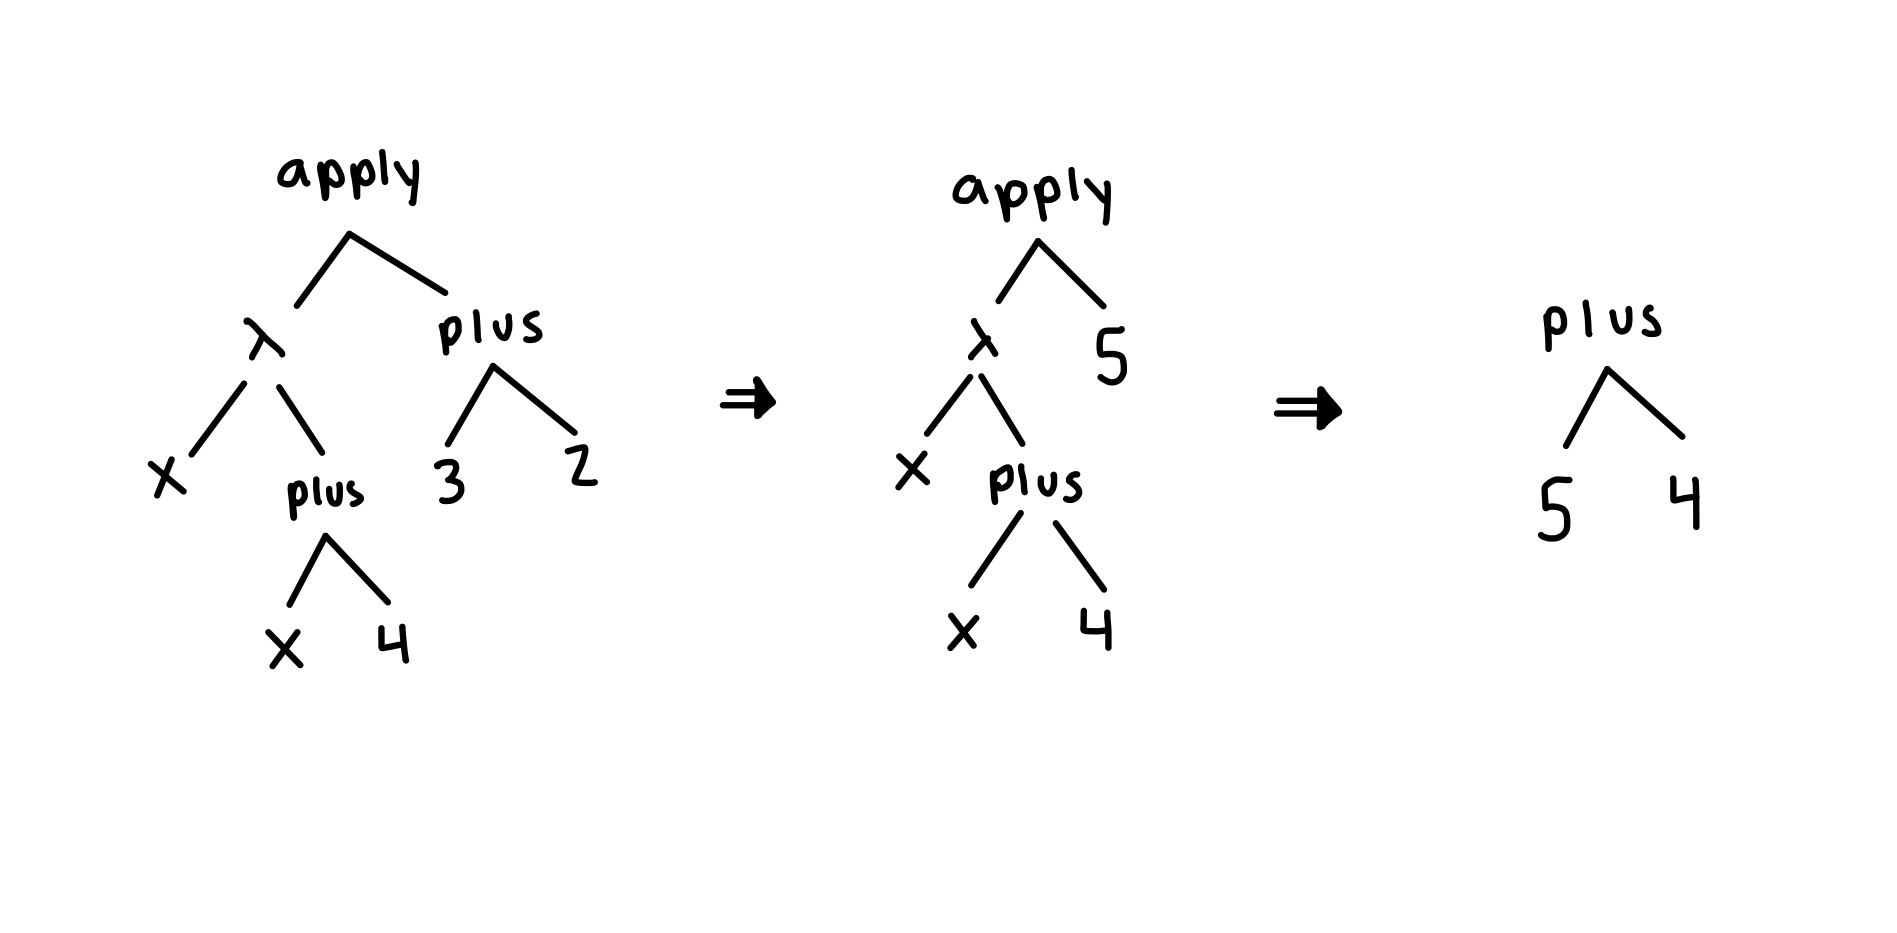
\includegraphics[width=16cm]{Example2Simplified.jpg}
    \caption{Lambda Example 2 Simplified}
    \label{fig:Lambda Example 2 Simplified}
\end{figure}

\medskip\noindent
Lambda just a early base version of computing and with these examples we have gone over what it means to use functions to evaluate. Although it might seem like a lot of work for a simple 2+3+5 but from a logical standpoint it is necessary especially when you start creating huge arguments and more demanding. 

\medskip\noindent
When expanding in Lambda Calculus you must learn about scoping. There are two types of variables when it comes to this. A bound variable which is a variable that is associated with a lambda while a free variable is one that is not associated with any lambda.

\medskip\noindent
Lets take our example from earlier and replace the ints with variables. 
$$ (\lambda x.x)(\lambda y.x)y$$

\medskip\noindent
This is how we would define these variables.

\medskip\noindent 
\begin{figure}[htp]
    \centering
    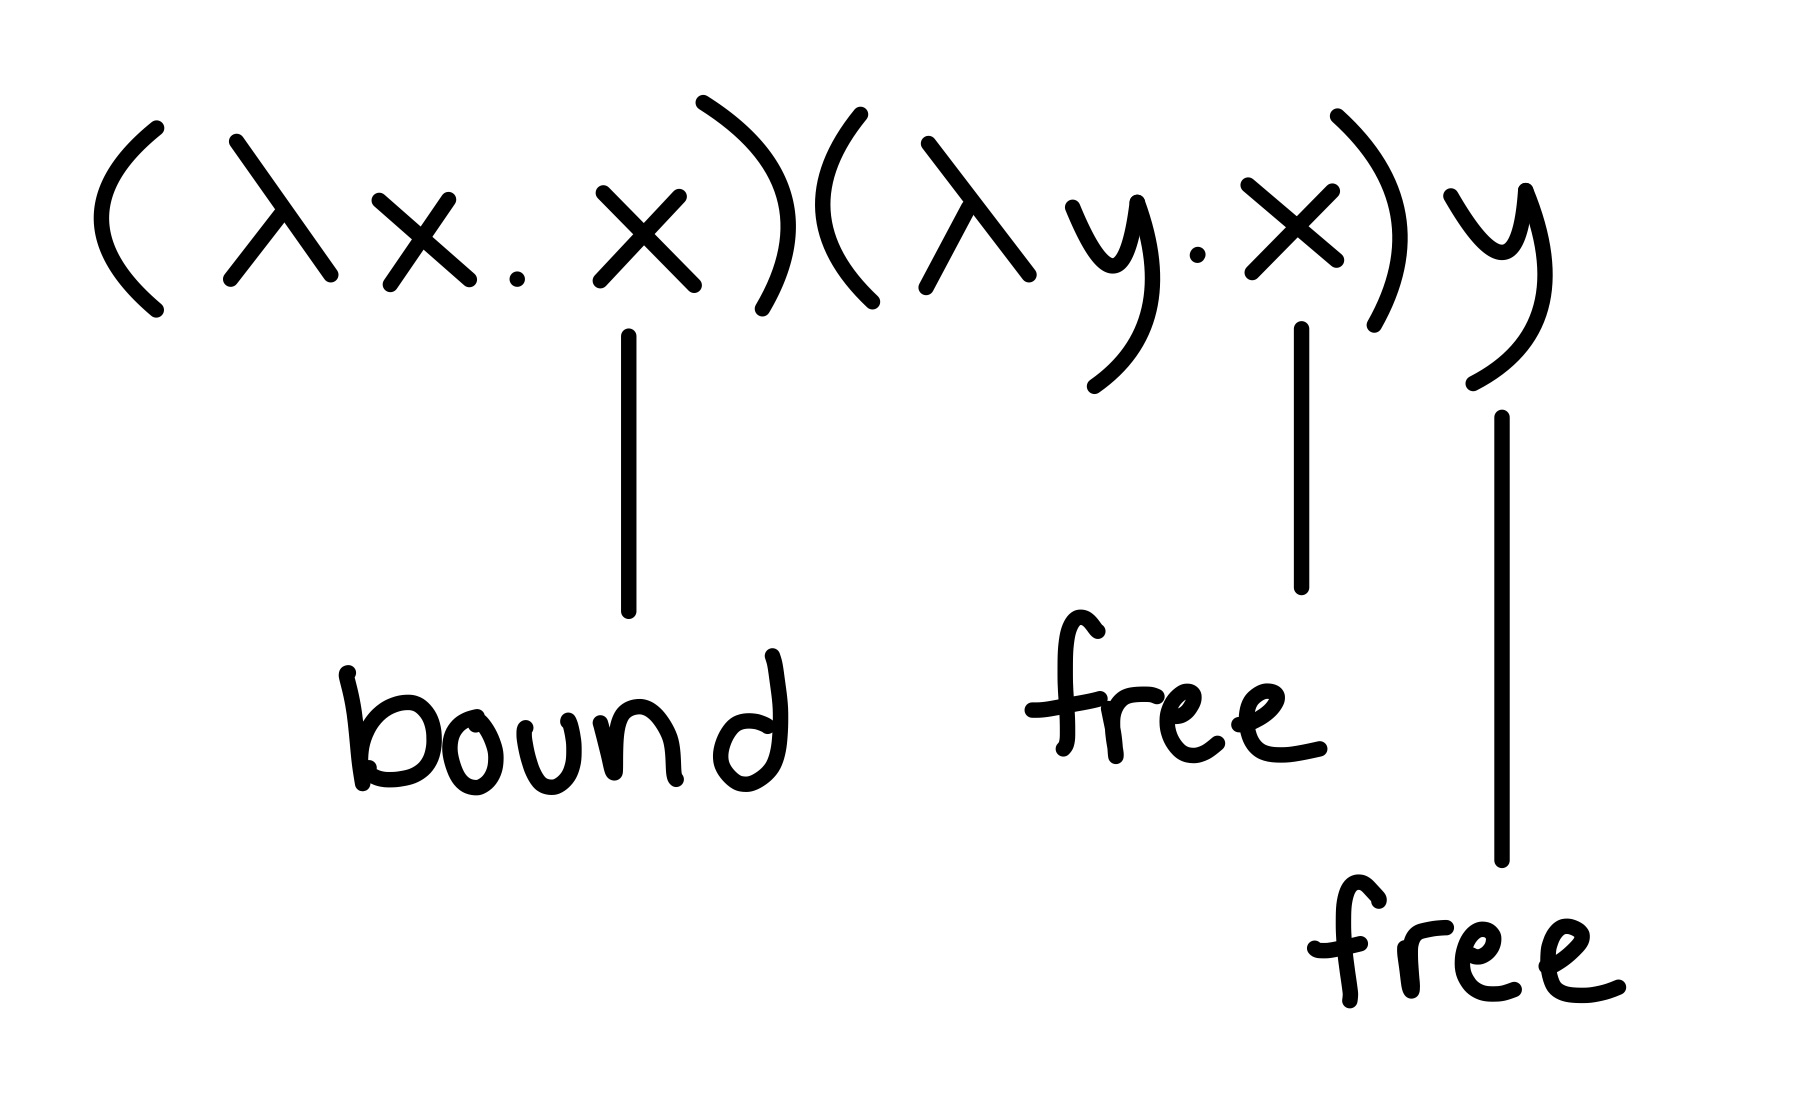
\includegraphics[width=7cm]{IMG_0680.jpg}
    \caption{Free and Bound Variables}
    \label{fig:Free and Bound}
\end{figure}

\medskip\noindent
A variable can appear twice in the same expression which can be seen above but depending on the situation it is in it can be bound but also free.

\medskip\noindent
This is a great way to understand what variables are dependent on especially with different functions. 

\subsection{Church encoding}

\medskip\noindent
So how one represents data in Lambda notation is called "Church encoding" and what is used to represent natural numbers is called "Church numerals." Lambda was actually created in the 1930's by a man named Church. 

\medskip\noindent
In lambda there are no ints or booleans, the only thing that is recognized is functions as this is not intended to have a practical implications. Its just to show that specific data types are not needed to show calculations. \cite{CEN}

\medskip\noindent
To transform these expressions in to actual data types you would need to add additional functions such as the + sign as we talked about a plus function earlier. Pure Lambda Calculus does not have these such things as they were not originally intended to have. 

\medskip\noindent
When one is interpreting Lambda Calculus people look at it in a way called "Intensional equality". It basically means that it is a proposition, so that it can assume things using induction to prove. 

\medskip\noindent
We use lambda terms to represent functions, and to get to the normal form or finding the lambda term's value you preform reductions which can be seen in the parse trees earlier in the report.\cite{CEN}

\medskip\noindent
Under Church encoding there is a way to have natural numbers be represented in Lambda. This is called "Church Numbers."

\medskip\noindent
How this works is that Church Numbers are basically functions that take in two parameters. In Lambda Calculus it is defined as such "0 not applying the function at all, proceed with 1 applying the function once, 2 applying the function twice, 3 applying the function three times, etc."

\medskip\noindent 
\begin{figure}[htp]
    \centering
    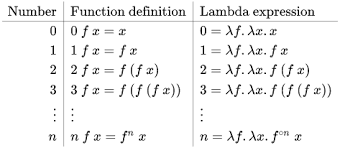
\includegraphics[width=10cm]{ChurchEncoding.png}
    \caption{Example of Church Numbers}
    \label{fig:Church Encodings}
\end{figure}
\cite{CEN}

\medskip\noindent
If we wanted to actually calculate with these rules the following chart shows how each expression would be evaluated.

\medskip\noindent 
\begin{figure}[htp]
    \centering
    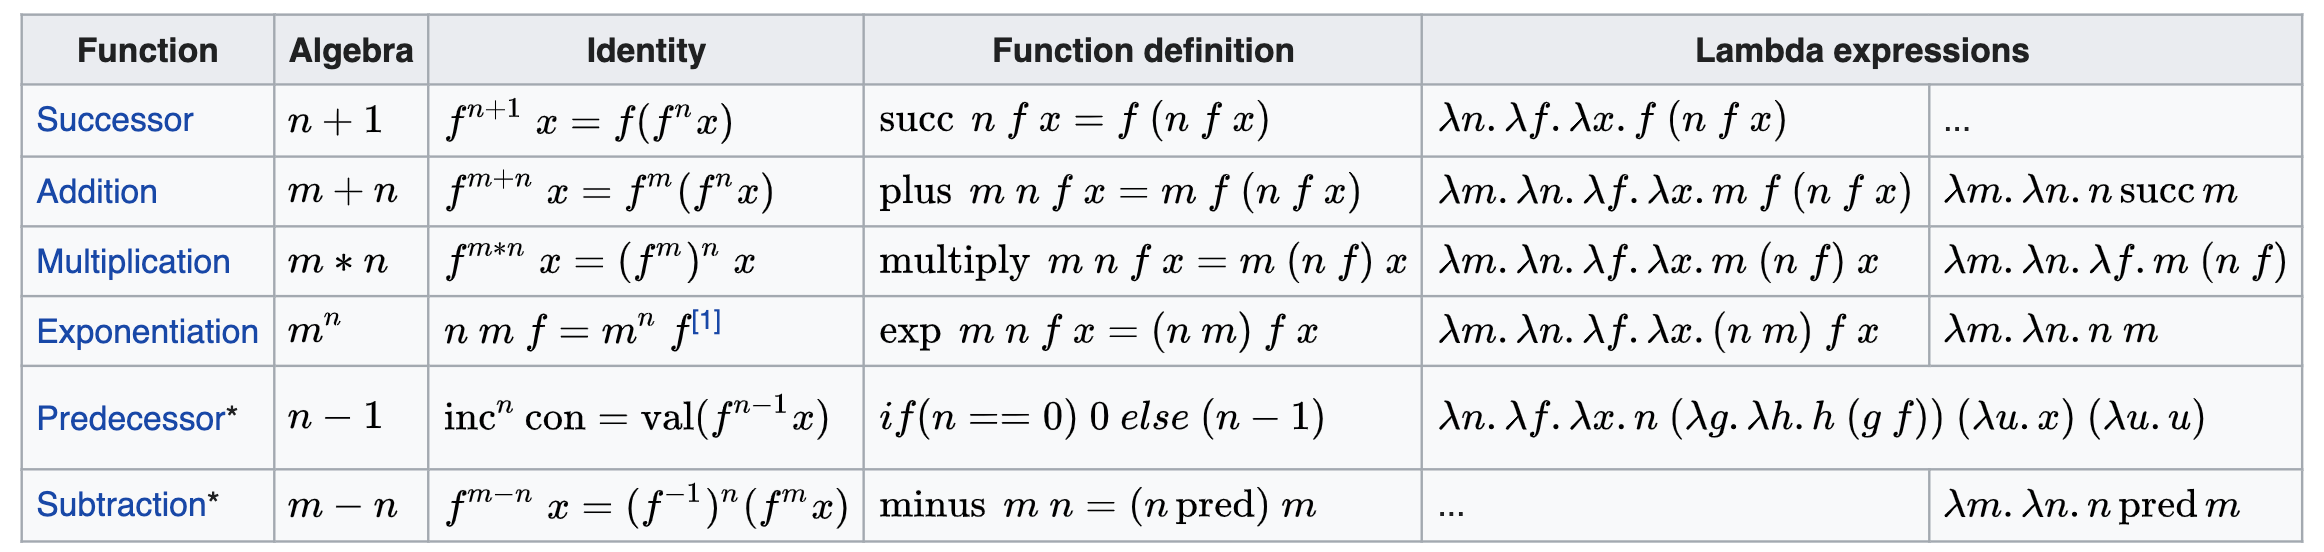
\includegraphics[width=17cm]{Church Numbers.png}
    \caption{Calculation of Church Numbers}
    \label{fig:Church Numbers}
\end{figure}
\cite{CEN}

\medskip\noindent
If we wanted to compute our plus one function from earlier it would look like.
$$ plusOne = \lambda n.\lambda f. \lambda x. f (n f x)$$

\medskip\noindent
In the table above it is called succession but is the same as plus one. 

\medskip\noindent
Using this Church Encoding we can do more with lambda calculus as a functional language than just evaluating functions.

\subsection{In-Class Application}

\medskip\noindent 
We created our own parser in Assignment 2 for Lambda Calculus. In the folder grammar, we have LambdaNat which at first is just a simple languages with "Prog.", "EAbs.", "EApp.", and "EVar.". But as we went on we further developed the language with other mathematical expressions, all with our lambda language. 

\medskip\noindent
In this grammar file, we were quite literally creating the grammar that is used to create the language, everything must be defined from how to create comments to what to write for equal.

\medskip\noindent
From there we created a parse which allowed us to compile our own code. 

\section{Project}

\medskip\noindent 
For my project I decided that I would attempt to create a working interface for our calculator app (Assignment 1). 

\subsection{Correcting Assignment 1}

\medskip\noindent 
The first part of my project was to fix my first assignment 1. My original assignment one had Non-exhaustive patterns which prohibited my code from working correctly it also was missing one of the required operation. 

\medskip\noindent 
I fixed my numbers.cf file, with some guidance from Curren Taber and Dan Hub, to have all the operations made sense and adding the missing ones as well. One thing that was not in my original assignment was parentheses. 

\medskip\noindent 
My new file's code looked like this below. 

\medskip\noindent 
\begin{lstlisting}
Plus. Exp ::= Exp "+" Exp1 ;
Minus. Exp ::= Exp "-" Exp1 ;
Times. Exp1 ::= Exp1 "*" Exp2 ;
Divide. Exp1 ::= Exp1 "/" Exp2 ;
Mod. Exp1 ::= Exp1 "%" Exp2 ;
Power. Exp2 ::= Exp2 "^" Exp3 ;
Negate. Exp3 ::= "-" Exp4 ;
UMinus. Exp4 ::= "-" Exp3 ;
Parentheses. Exp4 ::= "(" Exp ")" ;
Abs. Exp4 ::= "|" Exp "|" ;
Max. Exp ::= Exp ">" Exp1 ;
Min. Exp ::= Exp "<" Exp1 ;
Num. Exp4 ::= Integer ;
coercions Exp 4 ;
\end{lstlisting}

\medskip\noindent 
Since I went and corrected this, I needed to go back to my interpreter to implement the new operations into my interpreter. 

\medskip\noindent 
\begin{lstlisting}
module Interpreter where

import AbsNumbers

eval :: Exp -> Integer
eval (Num n) = n
eval (Plus n m) = (eval n) + (eval m)
eval (Minus n m) = (eval n) - (eval m)
eval (Times n m) = (eval n) * (eval m)
eval (Divide n m) = (eval n) `div` (eval m)
eval (UMinus n) = - (eval n)
eval (Mod n m) = (eval n) `mod` (eval m)
eval (Power n m) = (eval n) ^ (eval m)
eval (Max n m) | (eval n) > (eval m) = (eval n) | (eval n) < (eval m) = (eval m)
eval (Min n m) | (eval n) > (eval m) = (eval m) | (eval n) < (eval m) = (eval n)
eval (Abs n) = abs (eval n)
\end{lstlisting}

\medskip\noindent
I made sure to test and run the program and once I was confident that it worked I moved on to the interface portion of my project.

\subsection{Creating an Interface}

\medskip\noindent
I did some research online before choosing what type of interface I wanted to create for this app or even where I wanted to have the application be able to be accessed from. 

\medskip\noindent
This class was very challenging for me as my specialty interest in computer science is UX/UI design so I thought trying to make this program into an application or at least have a visual aspect would be very fun.

\medskip\noindent
At first I looked into making this project into an iOS app as it is something I enjoy doing but ran into a few difficulties as Xcode uses swift and would not be able to implement something in Haskell. 

\medskip\noindent
I came across this website called IHP \cite{IHP}. It is has a web-based schema design and works with Haskell projects!

\medskip\noindent
They had a few projects that used their platform to create full fledged apps using Haskell! I will link a some of these examples as they were very interesting to look at and were super informative. 

\medskip\noindent
\href{https://co2db.ihpapp.com}{CO2 Database} is a project that uses this site to create an interface to look up C02 producers. The \href{https://github.com/philschonholzer/co2db}{GitHub} for the project is public and was very interesting to look at just because the topic is very interesting but now I have more of an understanding of Haskell and better read the program.

\subsection{Issues and Problems}
Unfortunately I was not able to get a working version of my code to work and create a successful interface. The code I worked on used GitPod to edit the code and unfortunately did not save when I pushed back to github. The more I looked into the issue I found that the site was down.

\medskip\noindent 
\begin{figure}[htp]
    \centering
    
\includegraphics[width=10cm]{Error Message.png}
    \caption{GitPod Error Message}
    \label{fig:GitPod}
\end{figure}

\medskip\noindent 
 This was okay as I did not get far into the code as I wanted to have user input as it could be a working application that could be used live but I can provide pictures of what the web client looked like.
 
\medskip\noindent 
\begin{figure}[htp]
    \centering
    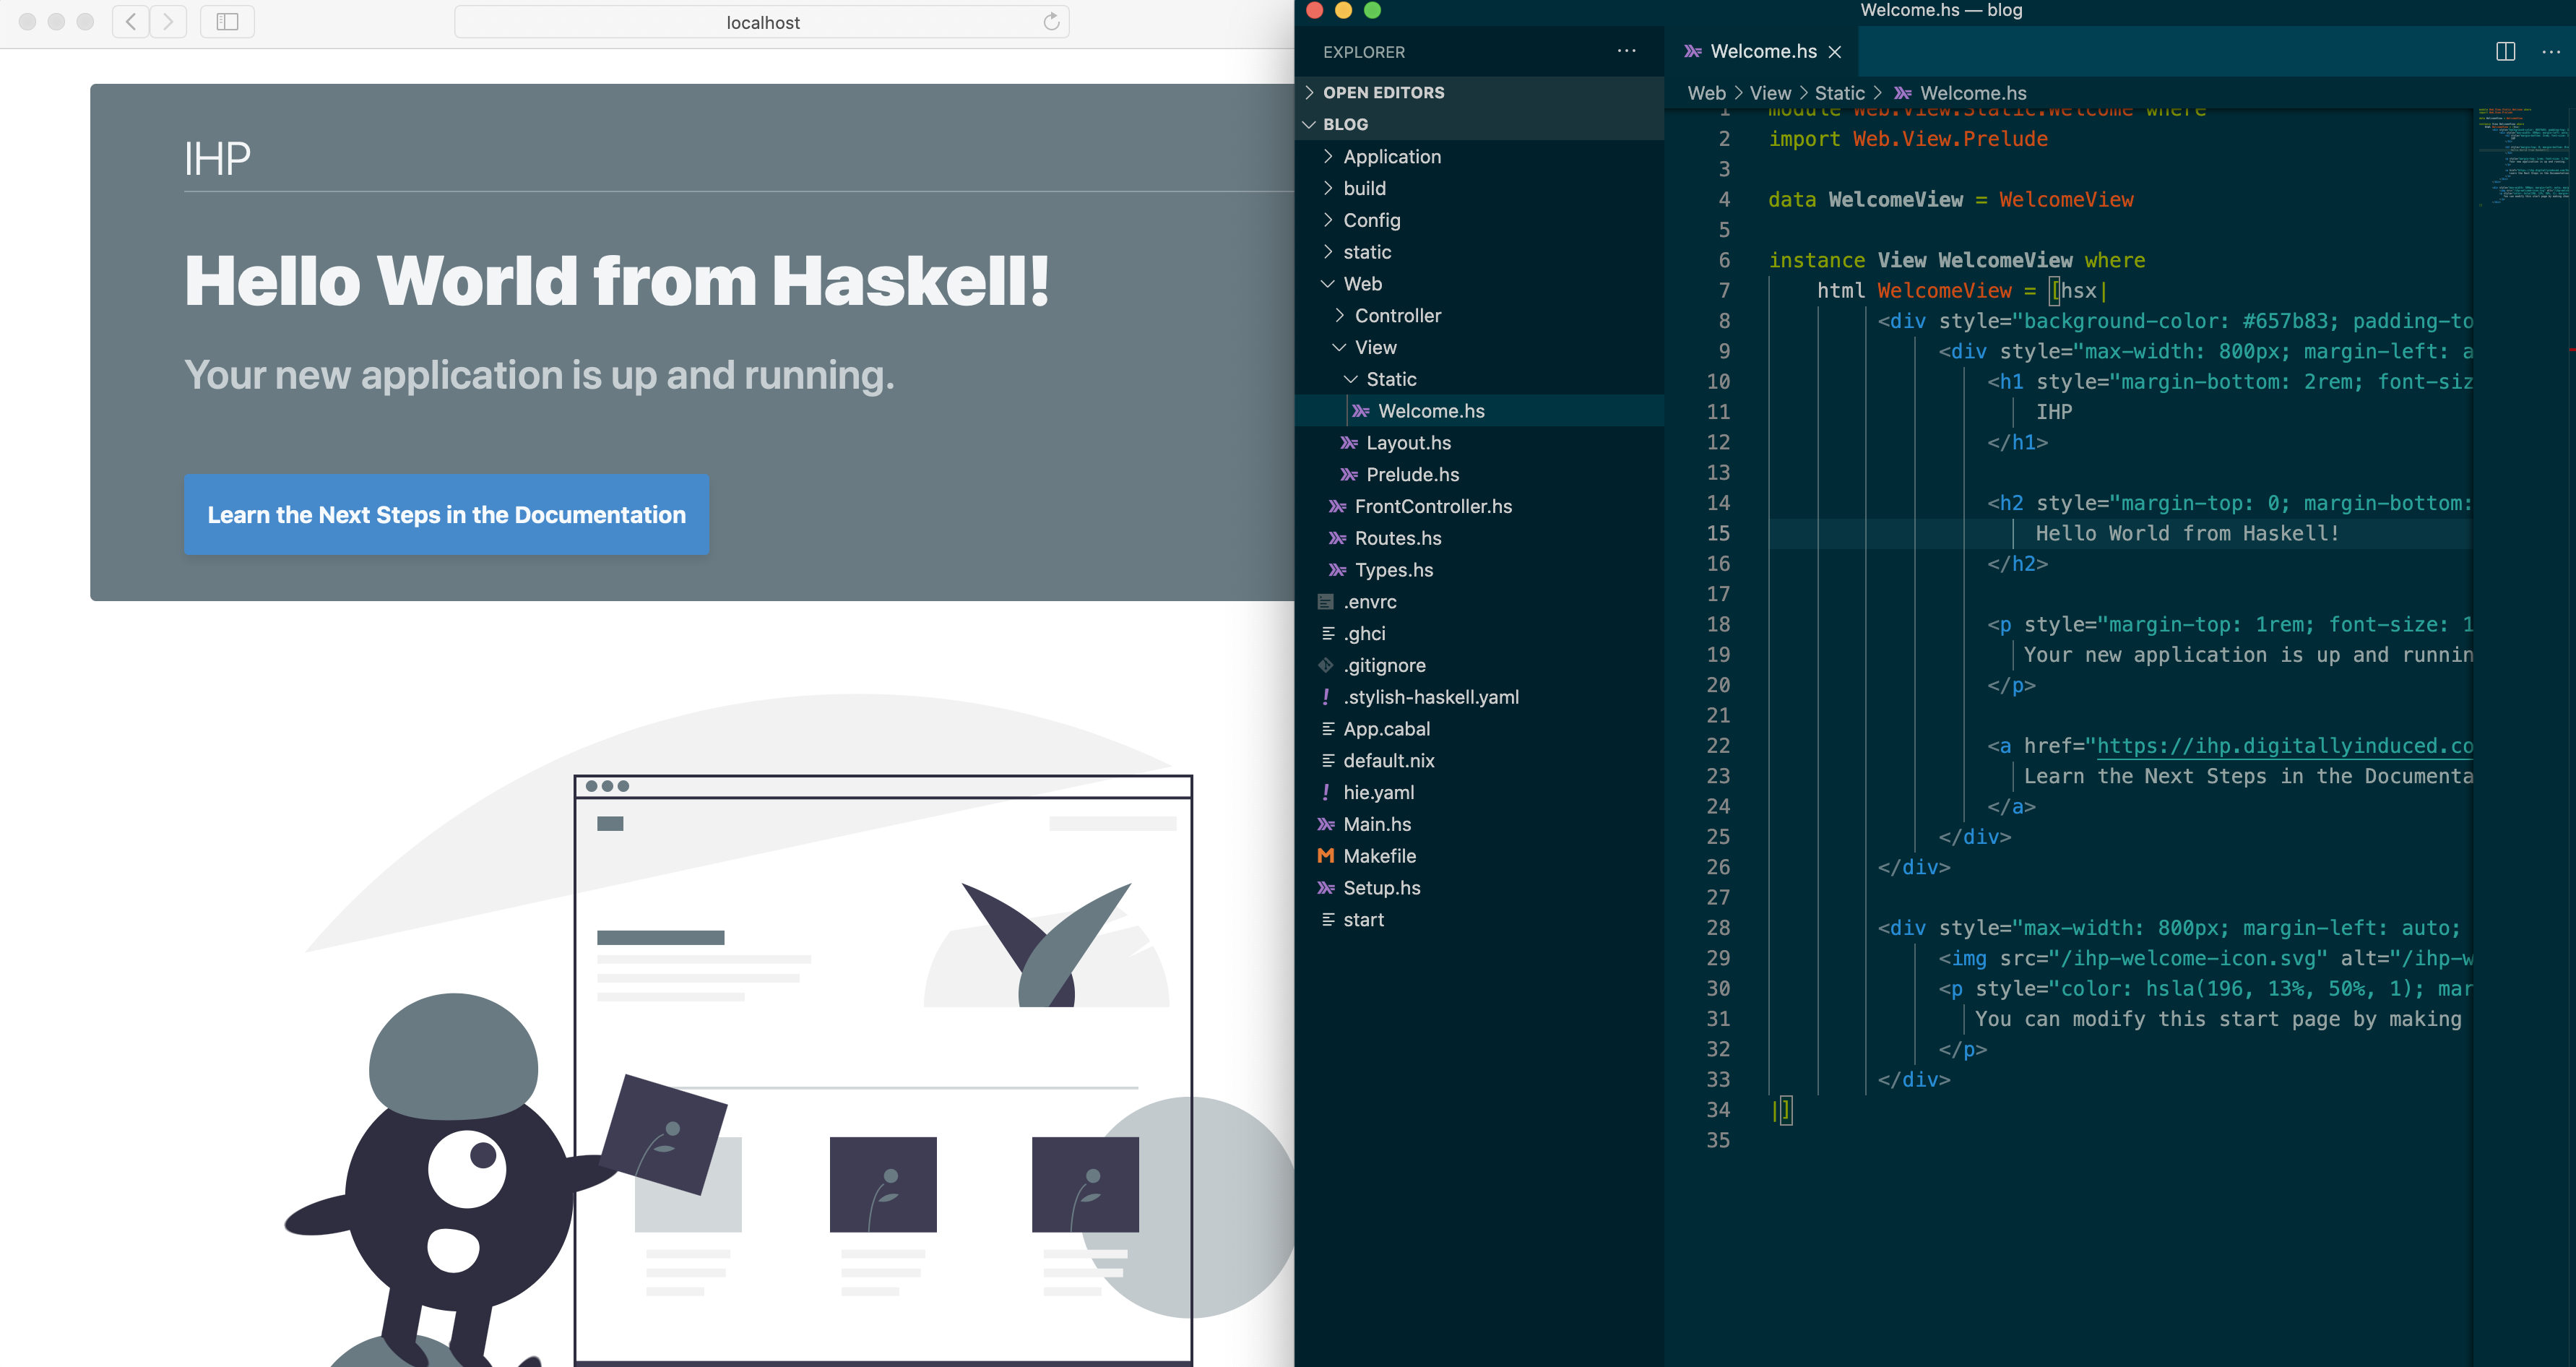
\includegraphics[width=17cm]{hello-world-2.png}
    \caption{Web Client with Editor open}
    \label{fig:Web Client with Editor open}
\end{figure}
\cite{IHP}

\medskip\noindent
Although I was not able to get my code to work, the website had a few examples of applications that were built in Haskell which were super informative! 

\medskip\noindent
When I do UI/UX design I usually use programs like Xcode or Unity and build off their build in functions, I learned that building a UI from scratch is VERY difficult ex. creating a website.

\subsection{Links to Repositories}
Here are my GitHub Repositories that were used for my project.

\medskip\noindent
\href{https://github.com/jkarstrom/ProgramingLanguages}{This is the link of my github repository} which has the template I had used to attempt to make an interface for this project. You can also use this link \url{https://github.com/jkarstrom/ProgramingLanguages}

\medskip\noindent
\href{https://github.com/bugster2010/Assignments354/tree/main/Assignment1}{This is the link of my github repository} which has my corrected Assignment 1 in it. I corrected it on my old repository I had with my partner for the duration of the class. You can also use this link \url{https://github.com/bugster2010/Assignments354/tree/main/Assignment1}


\section{Conclusions}\label{conclusions}
In this paper we have gone over the basis of the purely functional programming language Haskell and how it differs from other languages that programmers use today. 

\medskip\noindent
In order to create your own language you must first create the grammar of your language and decide how things will be evaluated, once you have that you create your own parser to compile and run files created in said language.

\medskip\noindent
Although that is very simply said it is actually very difficult to implement and takes a lot of logistic planning.

\subsection{Take Away}
This course was extremely difficult not in an there was a lot of work or assignments but in a this is very difficult material type of way.

\medskip\noindent 
We learnt a whole new programming language that I had never used before and not to mention we tackled building projects that we have not done in other classes before. Although it was very difficult it was very rewarding learning about the basics of programming and how deeply connected the theories are to math and research. 

\medskip\noindent 
The report in the end was a lot of work but I feel like I have a better grasp of what we learned. Doing more research on the subject and not keeping to what was in the talked about in the class and instead looking at things that interested me more I definitely had a more productive learning curve of the material.

\medskip\noindent 
This is a very important class that I believe all programmers should take no matter if they will work with the grammar of languages, the logic behind the languages is something that has definitely opened my eyes about the languages that I use day to day.

\begin{thebibliography}{99}
\bibitem[PL]{PL} \href{https://github.com/alexhkurz/programming-languages-2021/blob/main/README.md}{Programming Languages 2021}, Chapman University, 2021.
\bibitem[IHP]{IHP} \href{https://ihp.digitallyinduced.com}{IHP}{}
\bibitem[HHP]{HHP} \href{https://riptutorial.com/haskell}{Haskell Remarks}{}
\bibitem[PLIN]{PLIN} \href{https://hackmd.io/@alexhkurz/Hk86XnCzD}{Programming Languages 2021}, Chapman University, 2021.
\bibitem[LP]{LP} \href{https://medium.com/background-thread/what-is-lazy-evaluation-programming-word-of-the-day-8a6f4410053f}{What is Lazy Evaluation?}{ Sept. 28, 2018}
\bibitem[BHH]{BHH} \href{https://www.futurelearn.com/info/courses/functional-programming-haskell/0/steps/27218}{Brief History of Haskell}{}
\bibitem[PYT]{PYT} \href{https://docs.python.org/3/reference/grammar.html}{Python Grammar}{}
\bibitem[MF]{MF} \href{http://learnyouahaskell.com/recursion}{Recursion}{}
\bibitem[LNS]{LNS} \href{https://wiki.haskell.org/Lazy_vs._non-strict}{Lazy vs. non-strict}{ 5 April 2021}
\bibitem[RR]{RR} \href{https://www.merriam-webster.com/dictionary/recursion}{Recursion}{}
\bibitem[LFG]{LFG} \href{http://pages.cs.wisc.edu/~horwitz/CS704-NOTES/1.LAMBDA-CALCULUS.html}{Lambda Calculus}{}
\bibitem[HP]{HP} \href{https://serokell.io/blog/haskell-history}{Haskell History}{ August 23rd, 2019}
\bibitem[CEN]{CEN} \href{https://en.wikipedia.org/wiki/Church_encoding}{Church encoding}{}
\bibitem[PAR]{PAR} \href{https://serokell.io/blog/haskell-history}{Haskell. History of a Community-Powered Language}{ August 23rd, 2019}
\bibitem[NS]{NS} \href{https://wiki.haskell.org/Lazy_vs._non-strict}{Lazy vs. non-strict}
\bibitem[BSP]{BSP} \href{https://www.geeksforgeeks.org/bubble-sort/}{Bubble Sort}{ 24 Sep, 2021}
\bibitem[LH]{LH} \href{http://learnyouahaskell.com/introduction}{Learn You a Haskell}
\bibitem[BSS]{BSS} \href{https://www.geeksforgeeks.org/bubble-sort/}{Bubble Sort}{ 24 Sep, 2021}
\bibitem[LA]{LA} \href{https://plato.stanford.edu/entries/lambda-calculus/}{The Lambda Calculus}{ 24 Sep, 2021}
\bibitem[BSH]{BSH} \href{https://www.adrians-blog.com/2020/11/03/building-algorithms-with-haskell-bubble-sort/}{Building algorithms with Haskell}
\bibitem[AG]{AG} \href{https://www.geeksforgeeks.org/ambiguous-grammar/?ref=lbp}{Ambiguous Grammar}
\end{thebibliography}

\end{document}
